\documentclass[11pt]{article}
\usepackage[letterpaper,margin=1in]{geometry}
\usepackage{graphicx}
\usepackage{booktabs}
\usepackage{longtable}
\usepackage{amsmath,amssymb}
\usepackage{textcomp}
\usepackage[hidelinks]{hyperref}
\usepackage{caption}
\usepackage{float}
\usepackage{siunitx}
\usepackage{authblk}
\captionsetup{font=small,labelfont=bf}
\setlength{\parskip}{0.4em}
\setlength{\parindent}{0pt}

\title{\vspace{-2em}Multi-Omic Profiling Reveals Lac-Phe as a Substrate-Driven\\
Exerkine Independent of CNDP2 Activation}
\author[1]{Steven Hershman}
\author[2]{Claude Science}
\affil[1]{Independent Researcher}
\affil[2]{Anthropic}
\date{}

\begin{document}
\maketitle


\section*{Abstract}

N-lactoyl-phenylalanine (Lac-Phe) is an exercise-inducible, CNDP2-derived metabolite
that suppresses feeding and adiposity, yet it is annotated in no released MoTrPAC
metabolomics feature table. Returning to the raw mass-spectrometry files --- an extraction
orchestrated by Claude Science across a heterogeneous compute stack, running locally for
Agilent decoding and statistics while dispatching the x86-only Thermo vendor-reader step to
ephemeral Linux containers on Modal, with HTTP range requests replacing multi-gigabyte
downloads --- we recovered an ion at Lac-Phe's exact mass across all 19 PASS1B rat tissues.
A positive-control benchmark on twelve released metabolites reproduces their mass (11/12
within $\pm$5 ppm), retention time and training dose-response (r = 0.75), confirming the
pipeline is quantitatively faithful for Lac-Phe's chemical class. The training response is
transient (peaking at 1--4 weeks, decaying by week 8) and female-predominant, and --- on a
selection-free timecourse omnibus across all 19 tissues and both chromatographic platforms
--- is statistically robust only in the heart (q = 0.014); no tissue survives the stricter
selection-aware correction. We then asked whether CNDP2 itself is activated by training at
any layer protein abundance cannot see. It is not: across 8 tissues, 0 of 26
chromatin-accessibility peaks and 0 of 125 DNA-methylation clusters at the locus reach
significance --- including a strand-corrected promoter CpG island over the transcription
start site, the one feature a methylation switch would move --- while CNDP2 protein and its
modification sites are flat or, in liver, decreasing. Since the same tissues yield thousands
of training-responsive epigenetic features genome-wide, this convergent silence is a
positive result: Lac-Phe production is substrate-driven flux gated by local lactate and
phenylalanine, not CNDP2 induction. Because that logic makes molecular persistence the
tractable therapeutic lever, we triage an in-silico panel of hydrolysis-resistant analogs
through a computational funnel (quantum-chemical stability, pharmacophore alignment, ADMET,
docking) and confirm the two leads by Boltz-2 co-folding, nominating a 1,2,3-triazole
isostere. Identity is held at MSI Level 2 pending an authentic-standard, MS/MS-enabled
follow-up. By separating the substrate that drives this exerkine from the enzyme wrongly
assumed to gate it, these results reframe how a Lac-Phe-raising therapy should be built and
chart a concrete path toward exercise mimetics that could extend the metabolic benefits of
training to those unable to train.

\section*{1. Introduction}

The search for the molecular mediators of exercise has produced few candidates as
compelling as Lac-Phe. Identified by Li and colleagues as the top exercise-inducible
metabolite in mouse, human and racehorse plasma, Lac-Phe is a pseudodipeptide of
lactate and phenylalanine that suppresses food intake and reduces adiposity in
diet-induced obese mice without altering energy expenditure, and whose biosynthetic
ablation blocks the anti-obesity benefit of exercise training [Li 2022]. It is produced
not by a dedicated synthase but by the reverse-proteolysis activity of the cytosolic
dipeptidase CNDP2, first characterised as the generator of a broad family of N-lactoyl
amino acids [Jansen 2015]. The molecule now sits at the centre of an expanding
therapeutic story: metformin's effect on food intake and body weight is partly
Lac-Phe-dependent [Xiao 2024a; Scott 2024], and reviews increasingly treat Lac-Phe as a
shared exercise/metformin effector [Xiao 2024b].

The MoTrPAC (Molecular Transducers of Physical Activity Consortium) PASS1B rat study is
the most comprehensive molecular map of endurance-training adaptation assembled to date,
profiling transcriptome, proteome, post-translational modifications, chromatin
accessibility, DNA methylation and metabolome across roughly 19 tissues after 1, 2, 4
and 8 weeks of progressive treadmill training [Amar 2024; Schenk 2024]. Yet its
untargeted metabolomics reports only named, peak-picked features, and Lac-Phe is absent
from every released table. That absence poses two separate questions, which prior work
has tended to conflate. First, *is Lac-Phe actually present and training-responsive in
these tissues* --- answerable only by returning to the raw spectra. Second, and
mechanistically deeper, *if a training response exists, does it arise because CNDP2 is
turned up* --- through chromatin opening, promoter demethylation, increased protein, or
activating post-translational modification --- *or because the enzyme is simply handed
more substrate*.

We address both. Building on a raw-spectra reanalysis that recovered a Lac-Phe-mass ion
across all 19 tissues, we test the CNDP2-activation hypothesis directly against MoTrPAC's
epigenetic and proteomic layers --- assays that see regulation abundance cannot --- and we
interpret the resulting cross-tissue pattern through an organ-level source--sink model
assembled from the primary literature.

\section*{2. Results}

\subsection*{2.1 A Lac-Phe-mass ion is present across all 19 tissues, with a transient, tissue-restricted training response}

\begin{quote}\small \textbf{Two statistical bars.} A \textit{selection-free} test evaluates the whole training timecourse jointly (Kruskal--Wallis across weeks 0/1/2/4/8). A \textit{selection-aware} test takes the largest weekly increase per study and controls it against a 5,000-shuffle permutation null of the same statistic. We hold results to both bars throughout; their construction and rationale are in Methods.\end{quote}

Reading the raw Agilent QTOF \texttt{.d} and Thermo \texttt{.raw} files deposited on Metabolomics
Workbench, we extracted ion chromatograms at Lac-Phe's monoisotopic mass (C\textsubscript{1}\textsubscript{2}H\textsubscript{1}\textsubscript{5}NO\textsubscript{4};
[M$-$H]\textsuperscript{$-$} 236.0928, [M+H]\textsuperscript{+} 238.1074) directly from the profile data --- 18 reversed-phase
studies across 9 tissues (888 biological samples) and 10 HILIC-only tissues (492
samples); local statistics were combined with remote Linux containers only for the
x86-only Thermo vendor-format conversion, and multi-gigabyte downloads were avoided by
ZIP64 range-request extraction, all orchestrated end-to-end by an agentic analysis system
(Claude Science) (Methods). An ion within 5 ppm at a chromatographically consistent retention time is
detectable in every tissue. Four independent MS1 lines of evidence --- an
N-lactoyl-amino-acid family eluting in hydrophobicity order (Spearman $\rho$ = 0.86), a co-eluting
in-source [Phe$-$H]\textsuperscript{$-$} fragment that tracks the intact ion across samples at r = 0.96, a
matching isotope envelope, and a coherent adduct pattern --- place the assignment at a
defensible MSI Level 2 (probable structure), above the mass-only Level 3. The raw
negative-mode spectrum at the Lac-Phe apex (Figure 2) shows the intact [M$-$H]\textsuperscript{$-$}
and its co-eluting in-source fragment directly, alongside a built-in negative control ---
free lactate [Lac$-$H]\textsuperscript{$-$}, which is swamped by the bulk lactate pool and does
\textit{not} track the intact ion.

The training response, tested across the full timecourse (each week versus sedentary
control; sex-stratified; with a selection-aware permutation null because the natural
statistic is the largest weekly increase per study), is transient and tissue-restricted
(Figure 1). It peaks early --- plasma at week 1, heart at week 2, white adipose sustained
through week 4 --- and decays toward baseline by week 8. Where present it is
female-predominant. Stratifying every one of the 19 tissues by sex and graphing the
reversed-phase and HILIC platforms separately (Figure 3) shows the pattern holds across
the atlas: in each organ with a significant training \textit{increase} --- white adipose,
heart and plasma on reversed-phase, adrenal on HILIC --- the female peak effect meets or
exceeds the male, with females reaching p = 0.008 at their strongest week (plasma +0.75;
heart week 2 +0.95; white adipose week 4 +1.70 log\textsubscript{2} versus same-sex
control). Males clear significance in the same direction only in white adipose (+1.37,
p = 0.036) and adrenal, and are non-significant in plasma and heart. Both reversed-phase ionizations
rise together at
the same early week in plasma, heart, white adipose and liver --- orthogonal-chemistry
corroboration of a real analyte. A well-calibrated decoy panel (64 m/z; 3.1\% naive
false-positive rate) confirms the detection is not a mass-picking artifact. We held every tissue to both bars uniformly across the reversed-phase and HILIC platforms.
On the selection-free timecourse omnibus, the \textbf{heart} positive-mode signal is the one
training \textit{increase} that survives FDR correction across the 18 reversed-phase studies
(permutation q = 0.014). Three further tissues cross the omnibus threshold but not as increases:
kidney (reversed-phase positive) and colon (HILIC) are training-associated \textit{decreases} ---
the kidney signal consistent with its clearance role --- and the adrenal (HILIC) increase is not
corroborated by the in-source fragment and is interference-suspect. Under the selection-aware
permutation null the heart signal is nominal (p = 0.032) but does not survive FDR, and no tissue
clears q $<$ 0.10. We therefore report the heart as the robust responder and treat the concordant
plasma and white-adipose transients as hypothesis-generating.

\begin{figure}[H]\centering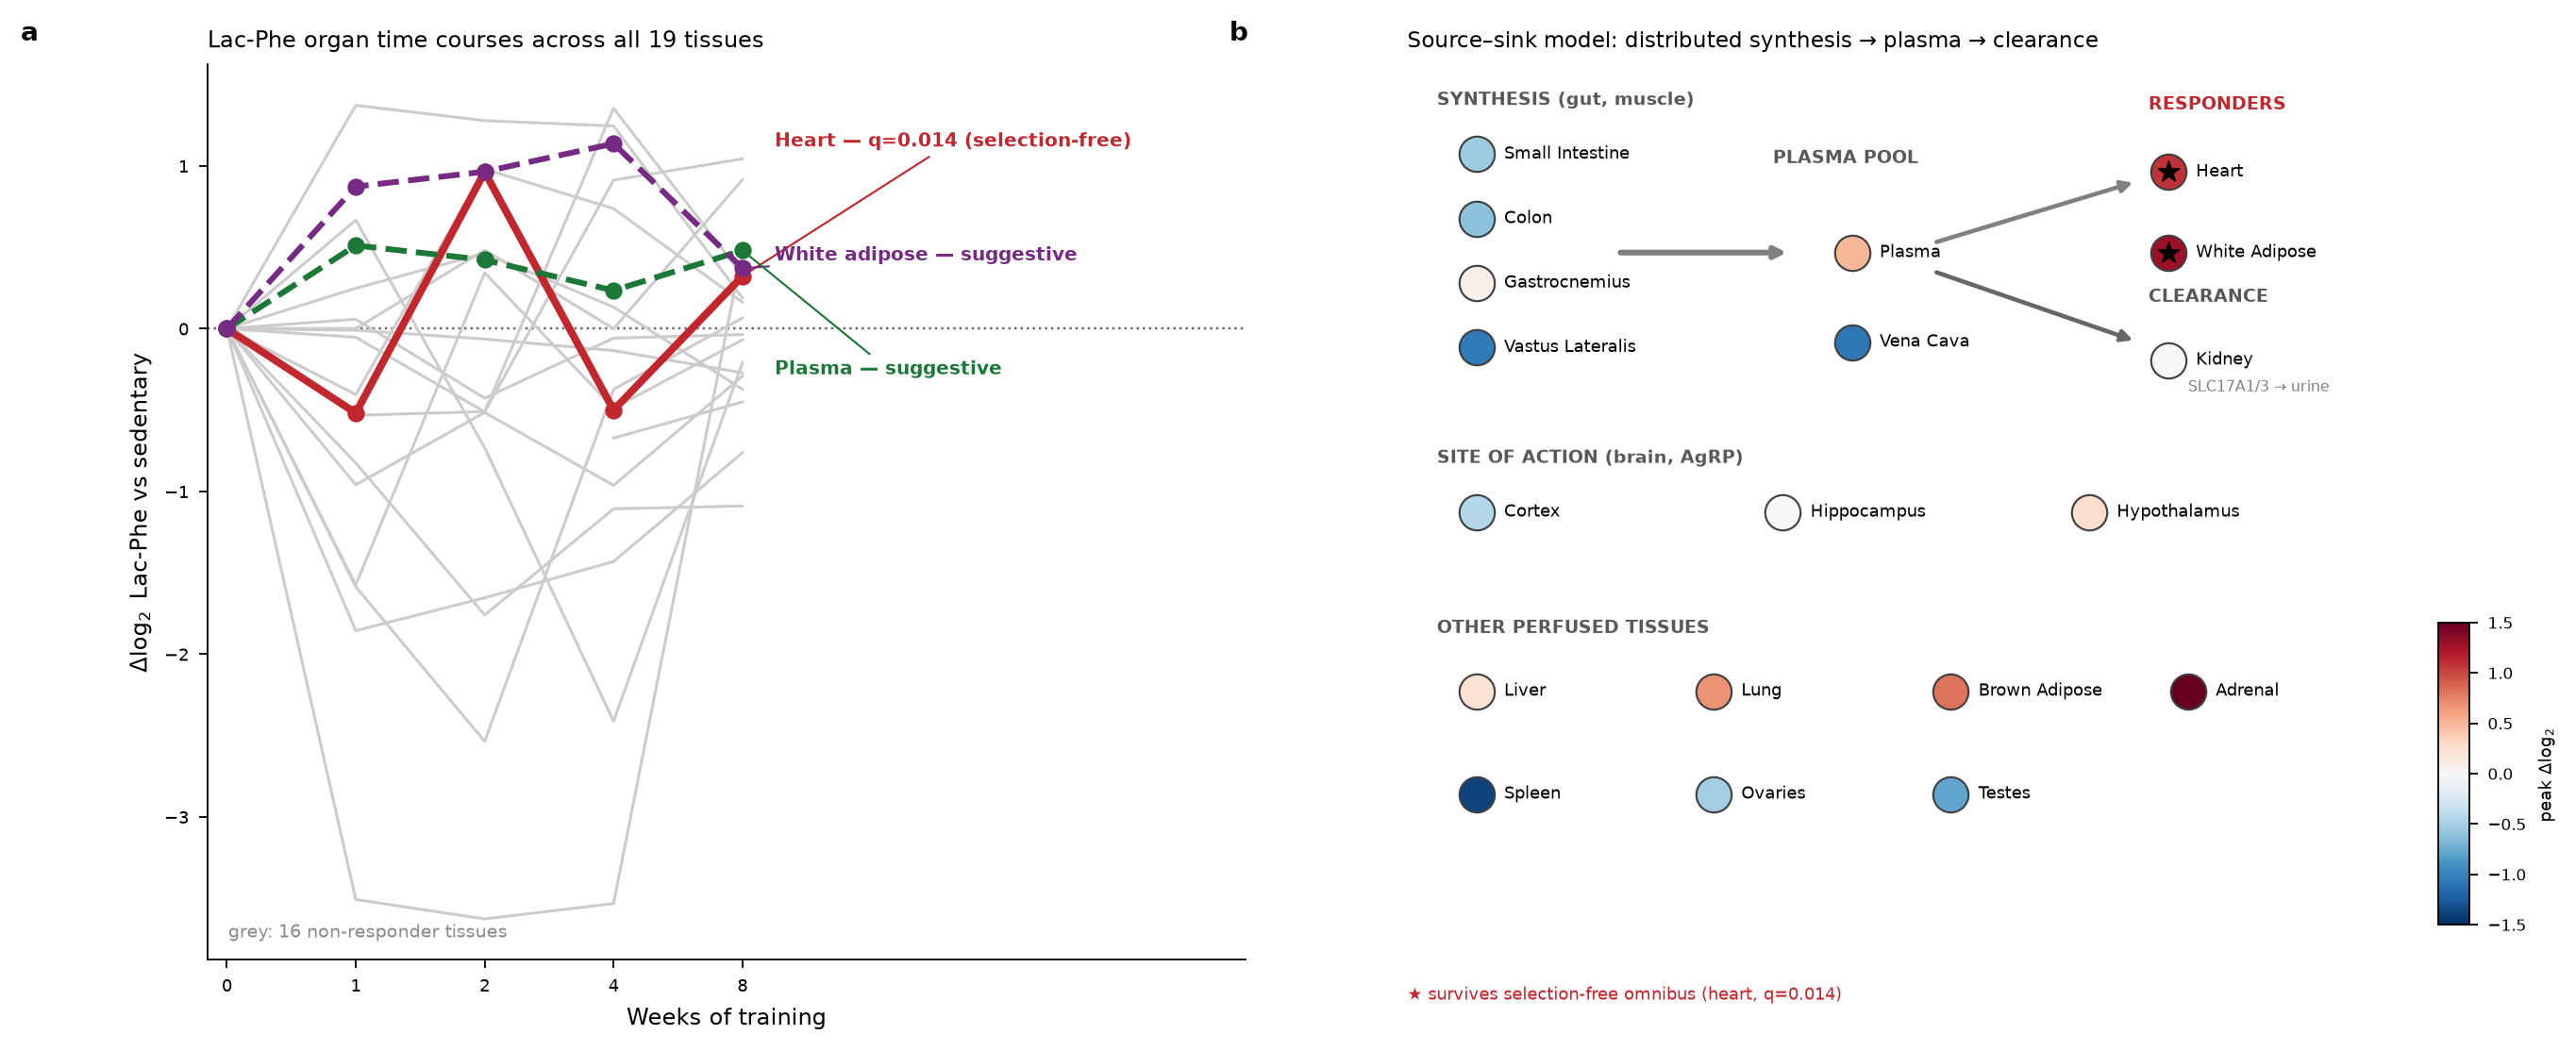
\includegraphics[width=\textwidth]{figures/figure1_organ_timecourse.png}\end{figure}

\textbf{Figure 1. A Lac-Phe-mass ion is present across all 19 tissues; the training response is transient and heart-restricted.} \textit{(a) $\Delta$log\textsubscript{2} Lac-Phe extracted-ion-chromatogram intensity versus sedentary control across weeks of training, shown for all 19 PASS1B tissues. The three statistically-supported responders are highlighted --- heart (red; the only tissue surviving the selection-free timecourse omnibus, q = 0.014) and plasma and white adipose (concordant, suggestive) --- with the remaining 16 tissues in grey. No tissue survives the stricter selection-aware correction. (b) The 19 organ responses mapped onto a source--sink model assembled from the literature: distributed CNDP2-mediated synthesis (gut, contracting muscle) feeds a circulating plasma pool sampled by all perfused tissues; nodes are coloured by peak $\Delta$log\textsubscript{2}, the two responders marked ($\star$); the kidney clears Lac-Phe to urine via SLC17A1/3; the brain (cortex, hippocampus, hypothalamus) is the site of anorexigenic action rather than a large metabolic pool. Production is substrate-driven, not CNDP2-induced. Sample sizes: n = 5 male + 5 female per training week per tissue (weeks 1/2/4/8) and n = 10 sedentary controls; 888 reversed-phase biological samples across 9 tissues (both ionization modes) plus 492 HILIC samples across 10 tissues, 1,380 samples across all 19 tissues.}

\begin{figure}[H]\centering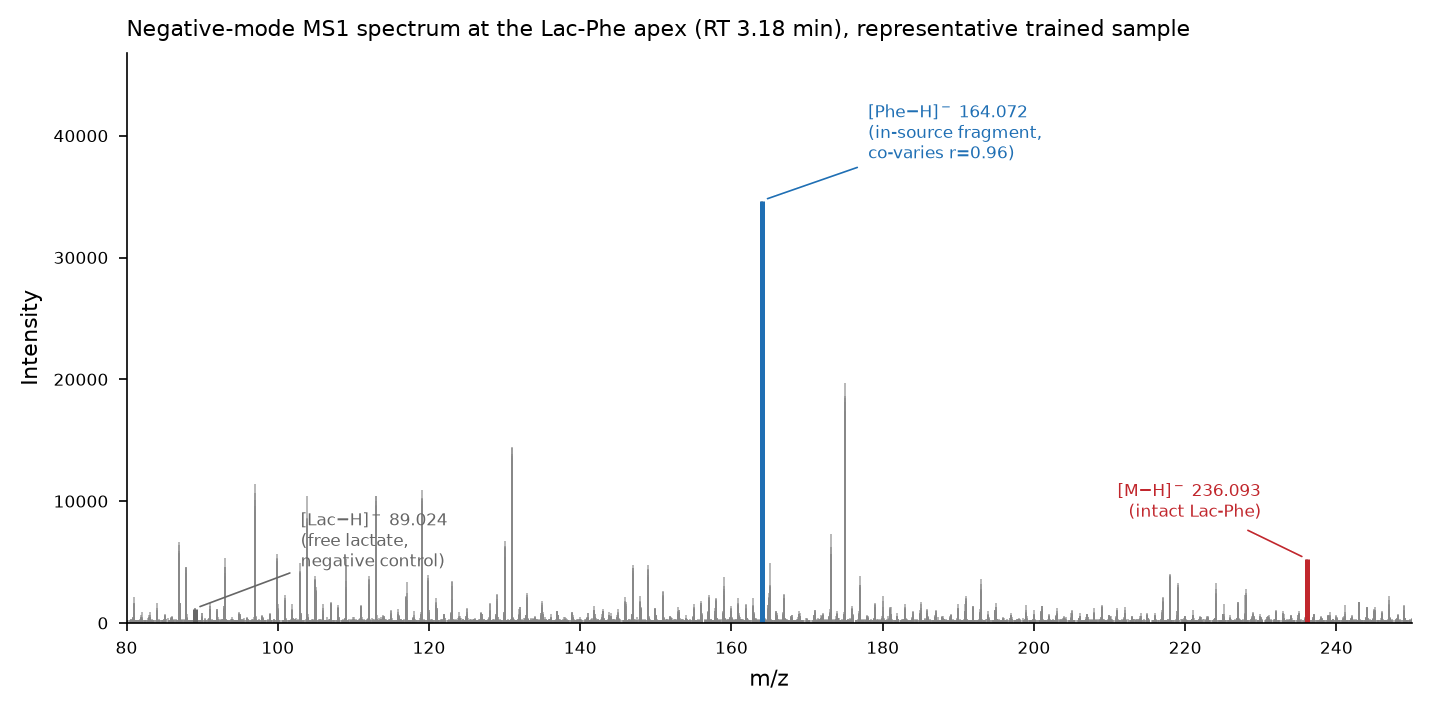
\includegraphics[width=0.82\textwidth]{figures/figure1c_spectrum.png}\end{figure}

\textbf{Figure 2. The raw negative-mode spectrum at the Lac-Phe apex resolves the intact ion, its diagnostic in-source fragment, and a built-in negative control.} \textit{Centroided MS1 spectrum ($m/z$ 80--250) at the validated Lac-Phe retention time (3.18 min) in a representative trained sample. The intact deprotonated molecule [M$-$H]$^-$ at $m/z$ 236.093 (red) and its in-source fragment [Phe$-$H]$^-$ at $m/z$ 164.072 (blue; neutral loss of the lactoyl C\textsubscript{3}H\textsubscript{4}O\textsubscript{2} moiety) co-elute and co-vary across the 50 biological samples (Spearman $\rho$ = 0.96, p = 4$\times$10\textsuperscript{$-$27}), the parent--fragment relationship a coincidental isobar cannot reproduce. Free lactate [Lac$-$H]$^-$ at $m/z$ 89.024 (grey), the other half of the molecule, serves as a built-in negative control: it is swamped by the large free-lactate pool and does not track the intact ion. These MS1 relationships, together with the retention-time--hydrophobicity ordering, the CNDP2-family co-variation and the isotope envelope, place the assignment at MSI Level 2; no MS/MS is available in the deposit (all scans are MS1) and Lac-Phe is absent from public spectral libraries.}

\begin{figure}[H]\centering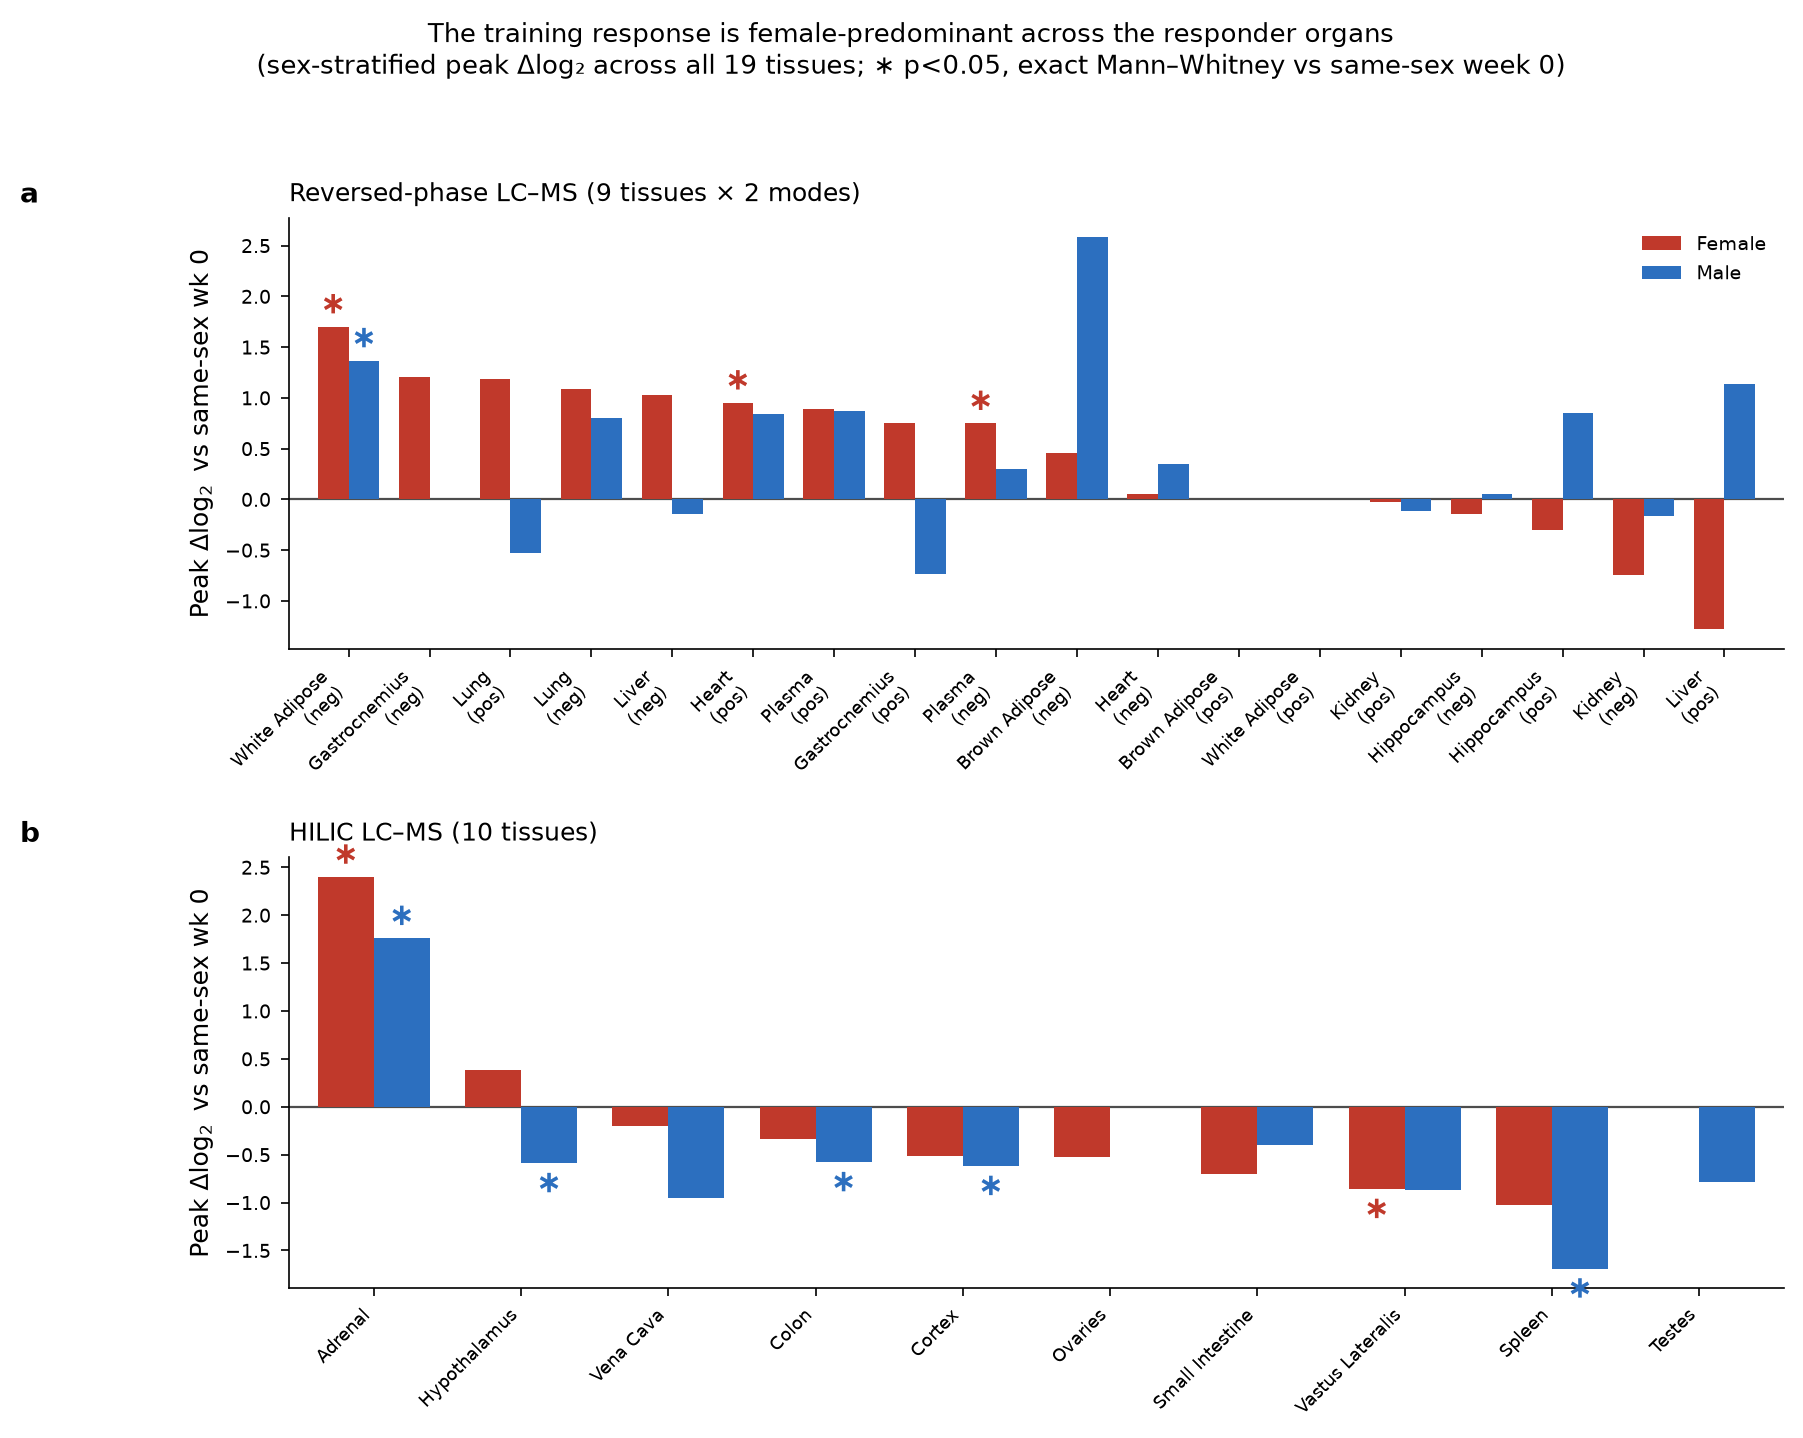
\includegraphics[width=\textwidth]{figures/figure2_sex_responders.png}\end{figure}

\textbf{Figure 3. The training response is female-predominant across the responder organs.} \textit{Sex-stratified peak $\Delta$log\textsubscript{2} Lac-Phe versus same-sex week-0 control across all 19 PASS1B tissues, with the two chromatographic platforms graphed separately: (a) reversed-phase LC--MS (9 tissues $\times$ 2 ionization modes) and (b) HILIC LC--MS (10 tissues). Each tissue$\times$mode is shown at its own peak week; bars are the female (red) and male (blue) peak effect. In every organ with a significant training increase --- white adipose, heart and plasma on reversed-phase, adrenal on HILIC --- the female effect meets or exceeds the male, and the two organs where males also clear significance (white adipose, adrenal) move in the same direction. Non-responding and decreasing tissues are shown for completeness. Sample sizes: n = 5 per sex per week (5 male + 5 female at each of weeks 0/1/2/4/8). $\ast$ p $<$ 0.05 (exact Mann--Whitney vs same-sex week-0 control).}

\subsection*{2.2 The raw-extraction pipeline reproduces MoTrPAC's own peak-picked metabolites}

Because the entire Lac-Phe result rests on a bespoke extraction that bypasses MoTrPAC's
production peak-picking, we validated that pipeline against a positive control: twelve
named metabolites that MoTrPAC \textit{did} release for plasma reversed-phase-negative
(ST002632), spanning the retention-time and abundance range (citrate, lactate, urate,
succinate, tyrosine, phenylalanine, tryptophan, hydroxyphenyllactic acid, phenylacetate,
ketoleucine, hydroxyindole acetate, indole lactate). We ran the identical extraction and
statistics on the same 50 biological raw files and compared against the consortium's
released values (Figure 4; Table 1).

The identity axes are essentially exact: the pipeline recovers every one of the twelve at
the released m/z (median mass error 11/12 within $\pm$5 ppm) and at the released retention
time (|$\Delta$RT| $\leq$ 0.03 min for 11/12). The single apparent outlier, tyrosine at $-$5.1 ppm
against the released reference, is not a pipeline error but a catch: MoTrPAC's own released
$m/z$ for tyrosine (180.0578) sits $\approx$49 ppm below the true [M$-$H]\textsuperscript{$-$} of
C\textsubscript{9}H\textsubscript{11}NO\textsubscript{3} (180.0666). The extraction faithfully
tracks the feature the consortium annotated as tyrosine; that feature (and the reference $m/z$
itself) is mis-specified in the flagship atlas, an error the raw-data reanalysis surfaces
rather than inherits. Per-sample abundance tracks the released values tightly for
well-resolved carboxylic acids --- Lac-Phe's own ion class --- with Pearson r = 0.97
(citrate), 0.99 (phenylacetate) and 0.60 (hydroxyindole acetate). Concordance is poor
only for metabolites expected to behave badly in this assay: phenylalanine, which ionizes
weakly in negative mode and sits near the detection floor (undetected in 12 of 50 samples);
lactate, which elutes at the void and shows low dynamic range; and tyrosine, whose released
reference is mis-annotated (above) so that neither series indexes the true molecule. The training-response quantity that
actually underlies our Lac-Phe claim --- the per-week $\Delta$log\textsubscript{2}FC dose-response --- reproduces at
Pearson r = 0.75 across the eleven metabolites detected in at least 45 of 50 samples
(44 metabolite-weeks; only phenylalanine, at 38/50, is excluded), with 73\% sign
agreement. Across all twelve without the detection filter the concordance is weaker
(r = 0.37), pulled down by the poorly-ionizing amino acids. The
pipeline is therefore quantitatively faithful for exactly the chemistry Lac-Phe belongs
to, and its failures fall on species with no bearing on the Lac-Phe assignment.

\begin{figure}[H]\centering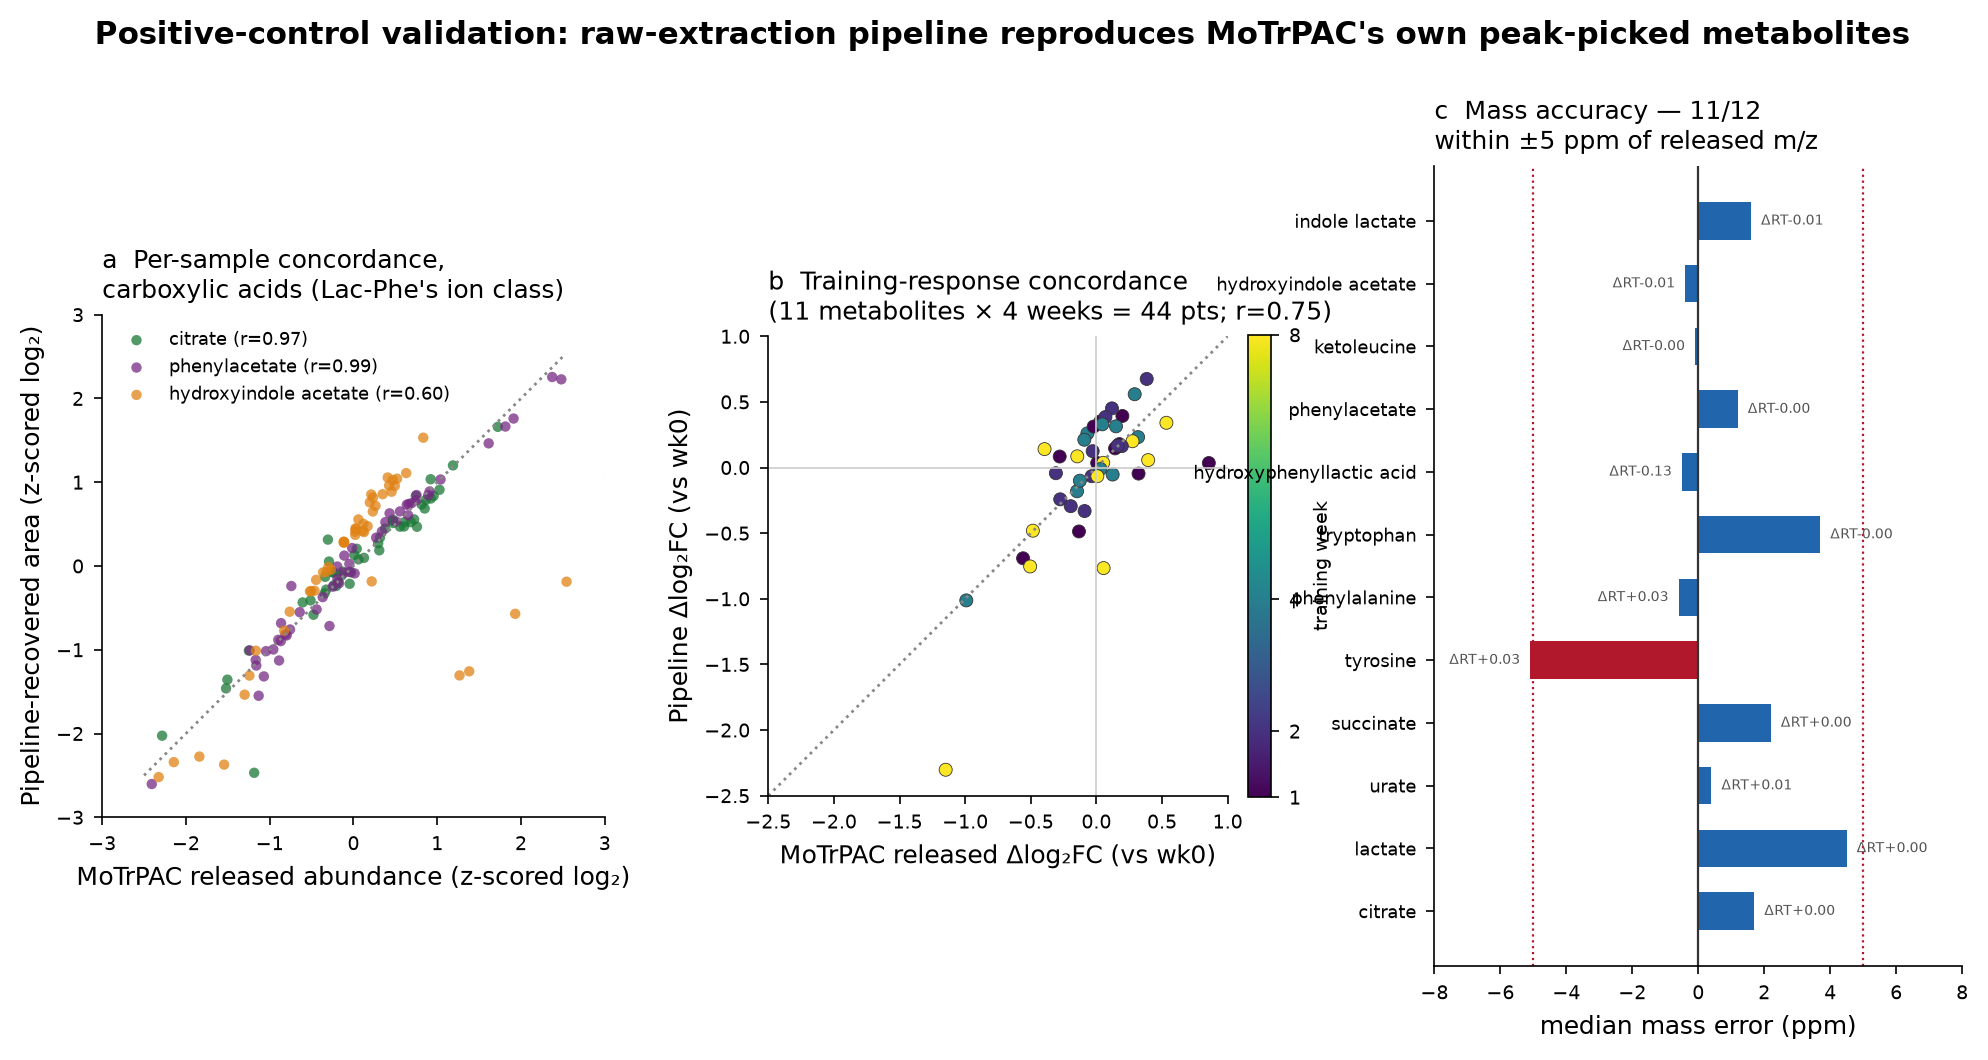
\includegraphics[width=\textwidth]{figures/figure3_positive_control.png}\end{figure}

\textbf{Figure 4. The raw-extraction pipeline reproduces MoTrPAC's own peak-picked metabolites.} \textit{(a) Per-sample concordance (z-scored log\textsubscript{2}) for three exemplar carboxylic acids in Lac-Phe's ion class; each point is one of 50 biological samples. (b) Training-response concordance: released versus pipeline-recovered $\Delta$log\textsubscript{2}FC (vs week 0) for the eleven reliably-detected metabolites ($\geq$45/50 samples) $\times$ 4 training weeks = 44 points, coloured by week (Pearson r = 0.75). (c) Mass accuracy for all twelve --- median mass error within $\pm$5 ppm of the released m/z for 11/12 (tyrosine $-$5.1); $\Delta$RT (min) annotated per metabolite. Same 50 raw plasma RP-neg files (ST002632) used for extraction and for MoTrPAC's released table.}

\textbf{Table 1. Positive-control concordance, twelve released metabolites (plasma RP-neg, ST002632).}

{\footnotesize\setlength{\tabcolsep}{4pt}
\begin{longtable}{llccccc p{1.7cm}}
\toprule
\textbf{Metabolite} & \textbf{Formula} & \textbf{Released m/z} & \textbf{RT (min)} & \textbf{Median ppm} & \textbf{Detected} & \textbf{Abund. r} & \textbf{Dir. agree} \\
\midrule\endhead
citrate & C6H8O7 & 191.0199 & 1.05 & +1.7 & 50/50 & 0.97 & 100\% \\
lactate & C3H6O3 & 89.0244 & 1.10 & +4.5 & 50/50 & 0.02 & 50\% \\
urate & C5H4N4O3 & 167.0211 & 1.26 & +0.4 & 50/50 & 0.44 & 100\% \\
succinate & C4H6O4 & 117.0189 & 1.51 & +2.2 & 50/50 & 0.50 & 50\% \\
tyrosine & C9H11NO3 & 180.0578 & 1.67 & $-$5.1 & 50/50 & $-$0.13 & 50\% \\
phenylalanine & C9H11NO2 & 164.0651 & 2.92 & $-$0.6 & 38/50 & $-$0.18 & 0\% \\
tryptophan & C11H12N2O2 & 203.0822 & 3.60 & +3.7 & 50/50 & 0.61 & 50\% \\
hydroxyphenyllactic acid & C9H10O4 & 181.0504 & 3.93 & $-$0.5 & 50/50 & 0.32 & 100\% \\
phenylacetate & C8H8O2 & 135.0448 & 4.05 & +1.2 & 50/50 & 0.99 & 100\% \\
ketoleucine & C6H10O3 & 129.0556 & 4.49 & $-$0.1 & 50/50 & 0.42 & 50\% \\
hydroxyindole acetate & C10H9NO3 & 190.0506 & 4.99 & $-$0.4 & 50/50 & 0.60 & 100\% \\
indole lactate & C11H11NO3 & 204.0606 & 5.49 & +1.6 & 48/50 & 0.14 & 50\% \\
\bottomrule
\end{longtable}
}

\textit{Abund. r = Pearson correlation of per-sample log\textsubscript{2} abundance (pipeline vs released). $\Delta$log\textsubscript{2}FC dir. agree = fraction of the four training weeks whose sign matches. Carboxylic acids (Lac-Phe's class) concord strongly; the three low-concordance rows are amino acids (weak RP-neg ionizers) and void-eluting lactate.}

\subsection*{2.3 CNDP2 is not epigenetically activated by training}

If training raised Lac-Phe by inducing CNDP2, the CNDP2 locus should show increased
chromatin accessibility or altered methylation --- most tellingly in the promoter and 5$'$
upstream region, where an exercise-inducible enhancer or a demethylating promoter CpG island
would be expected to appear. It does not (Figure 5, top). CNDP2 is a minus-strand gene on
rat chromosome 18 (RefSeq NM\_001010920; transcription start site at chr18:81,539,065, rn6),
so its promoter and upstream region lie at \textit{higher} genomic coordinates than the gene
body. MoTrPAC's ATAC-seq and RRBS assays map 26 accessibility peaks and 125 methylation
clusters across the locus; strand-aware annotation shows this coverage is not confined to the
gene body but extends 5$'$ into the promoter and upstream region to $\approx$15 kb (8 ATAC
peaks and 31 methylation clusters lie 5$'$ of the TSS). A canonical CpG island straddles the
CNDP2 promoter (chr18:81,538,627--81,539,249) and is densely tiled by RRBS
--- 31 features (1 ATAC peak, 30 methylation clusters) overlap it --- with a second CpG island
in the gene body. Not one of these 151 features, including every promoter, upstream and
CpG-island feature, reaches 5\% FDR for a training effect in any of the 8 assayed tissues
(BAT, heart, hippocampus, kidney, liver, lung, gastrocnemius, white adipose), at any
timepoint, in either sex --- confirmed both by their absence from the per-tissue
significance-filtered objects and by a direct cross-check against the consortium's timewise
differential-statistics set. The promoter CpG island, the region most likely to carry an
activating demethylation signal, is flat. This is not a power artifact: the same eight tissues
yield thousands of training-significant epigenetic features genome-wide (e.g. 1,032 liver ATAC
peaks, 621 BAT methylation clusters), and the heart --- the one tissue where the metabolite
signal is statistically robust --- has 75 significant ATAC peaks and 107 significant
methylation clusters, none at CNDP2.

\textbf{Table 2. CNDP2-locus ATAC-seq accessibility peaks, strand-corrected (rat chr18, rn6, minus strand; TSS = 81,539,065).} Positions are transcription-oriented: negative = 5$'$ upstream of the TSS (promoter direction), 0 = straddles the TSS, positive = into the gene body, ``3$'$ flank'' = beyond the 3$'$ end of the gene. None enters any tissue's 5\%-FDR training-significant set (8 tissues $\times$ 4 timepoints $\times$ 2 sexes). The three peaks previously mislabelled ``promoter-proximal'' ($-$1694/$-$1086/$-$632 bp) sit, under the correct minus-strand model, on the 3$'$ flank $\approx$18 kb from the TSS. Full per-peak coordinates are in \texttt{cndp2\_markers\_extended.csv}.

{\footnotesize
\begin{longtable}{llrll}
\toprule
\textbf{Peak (chr18, rn6)} & \textbf{Strand-corrected region} & \textbf{5$'$ dist. to TSS} & \textbf{CpG island} & \textbf{Training-sig?} \\
\midrule\endhead
81553938-81554348 & promoter / 5$'$ upstream & $-$15.3 kb & --- & not in 5\% set \\
81550370-81550604 & promoter / 5$'$ upstream & $-$11.5 kb & --- & not in 5\% set \\
81549788-81550107 & promoter / 5$'$ upstream & $-$11.0 kb & --- & not in 5\% set \\
81547707-81547962 & promoter / 5$'$ upstream & $-$8.9 kb & --- & not in 5\% set \\
81545865-81546091 & promoter / 5$'$ upstream & $-$7.0 kb & --- & not in 5\% set \\
81541253-81542171 & promoter / 5$'$ upstream & $-$3.1 kb & --- & not in 5\% set \\
81539307-81539553 & promoter / 5$'$ upstream & $-$0.5 kb & --- & not in 5\% set \\
81538463-81539274 & promoter (straddles TSS) & 0 & promoter CpG island & not in 5\% set \\
81522039--81535667 (15 peaks) & gene body & +3.4 to +17.0 kb & 1 in gene-body CpG isl. & not in 5\% set \\
81520888-81521336 & 3$'$ flank & $-$17.7 kb (3$'$) & --- & not in 5\% set \\
81520682-81520882 & 3$'$ flank & $-$18.2 kb (3$'$) & --- & not in 5\% set \\
81519349-81520274 & 3$'$ flank & $-$18.8 kb (3$'$) & --- & not in 5\% set \\
\bottomrule
\end{longtable}
}

\textbf{Table 3. CNDP2-locus RRBS methylation clusters, strand-corrected (125 clusters).} Region assignment uses tile-centre coordinates (RRBS clusters are reported by 500-bp tile; per-cluster bp bounds are not public). None is training-significant. Full annotation is in \texttt{cndp2\_markers\_extended.csv}.

\begin{longtable}{lrll}
\toprule
\textbf{Region (strand-corrected)} & \textbf{n clusters} & \textbf{Overlaps CpG island} & \textbf{Training-sig?} \\
\midrule\endhead
promoter / 5$'$ upstream (of TSS) & 8 & --- & 0 / 8 in 5\% set \\
promoter, straddling TSS & 23 & promoter CpG island & 0 / 23 in 5\% set \\
gene body & 94 & 25 in gene-body CpG island & 0 / 94 in 5\% set \\
\textbf{total} & \textbf{125} & \textbf{31 promoter, 25 gene-body} & \textbf{0 / 125} \\
\bottomrule
\end{longtable}

\textbf{Table 4. The CNDP2 null is not a power artifact --- genome-wide training-significant features in the same assays and tissues.}

\begin{longtable}{llll}
\toprule
\textbf{Tissue} & \textbf{Assay} & \textbf{Genome-wide sig. features} & \textbf{CNDP2 sig. features} \\
\midrule\endhead
Liver & ATAC & 1,032 & 0 \\
SkM-GN & ATAC & 442 & 0 \\
Heart & ATAC & 75 & 0 \\
Heart & RRBS methyl & 107 & 0 \\
BAT & RRBS methyl & 621 & 0 \\
\bottomrule
\end{longtable}


Annotating the locus with species-matched UniBind rat ChIP-seq (ENCODE contains no
\textit{Rattus norvegicus} experiments) explains why. The CNDP2 promoter and gene body are
dominated by constitutive hepatic/renal metabolic transcription factors --- Hnf4a (44
sites), the bile-acid receptor Nr1h4/FXR (18), the carbohydrate-response factor
Mlxipl/ChREBP, Tcf7l2 and Sp1. The only activity- or stress-inducible factors present
are AP-1/Jun (33 gene-body sites) and a single promoter Egr2 site. The locus is wired
for constitutive metabolic control, not for an exercise-inducible enhancer --- concordant
with the flat accessibility and methylation.

\begin{figure}[H]\centering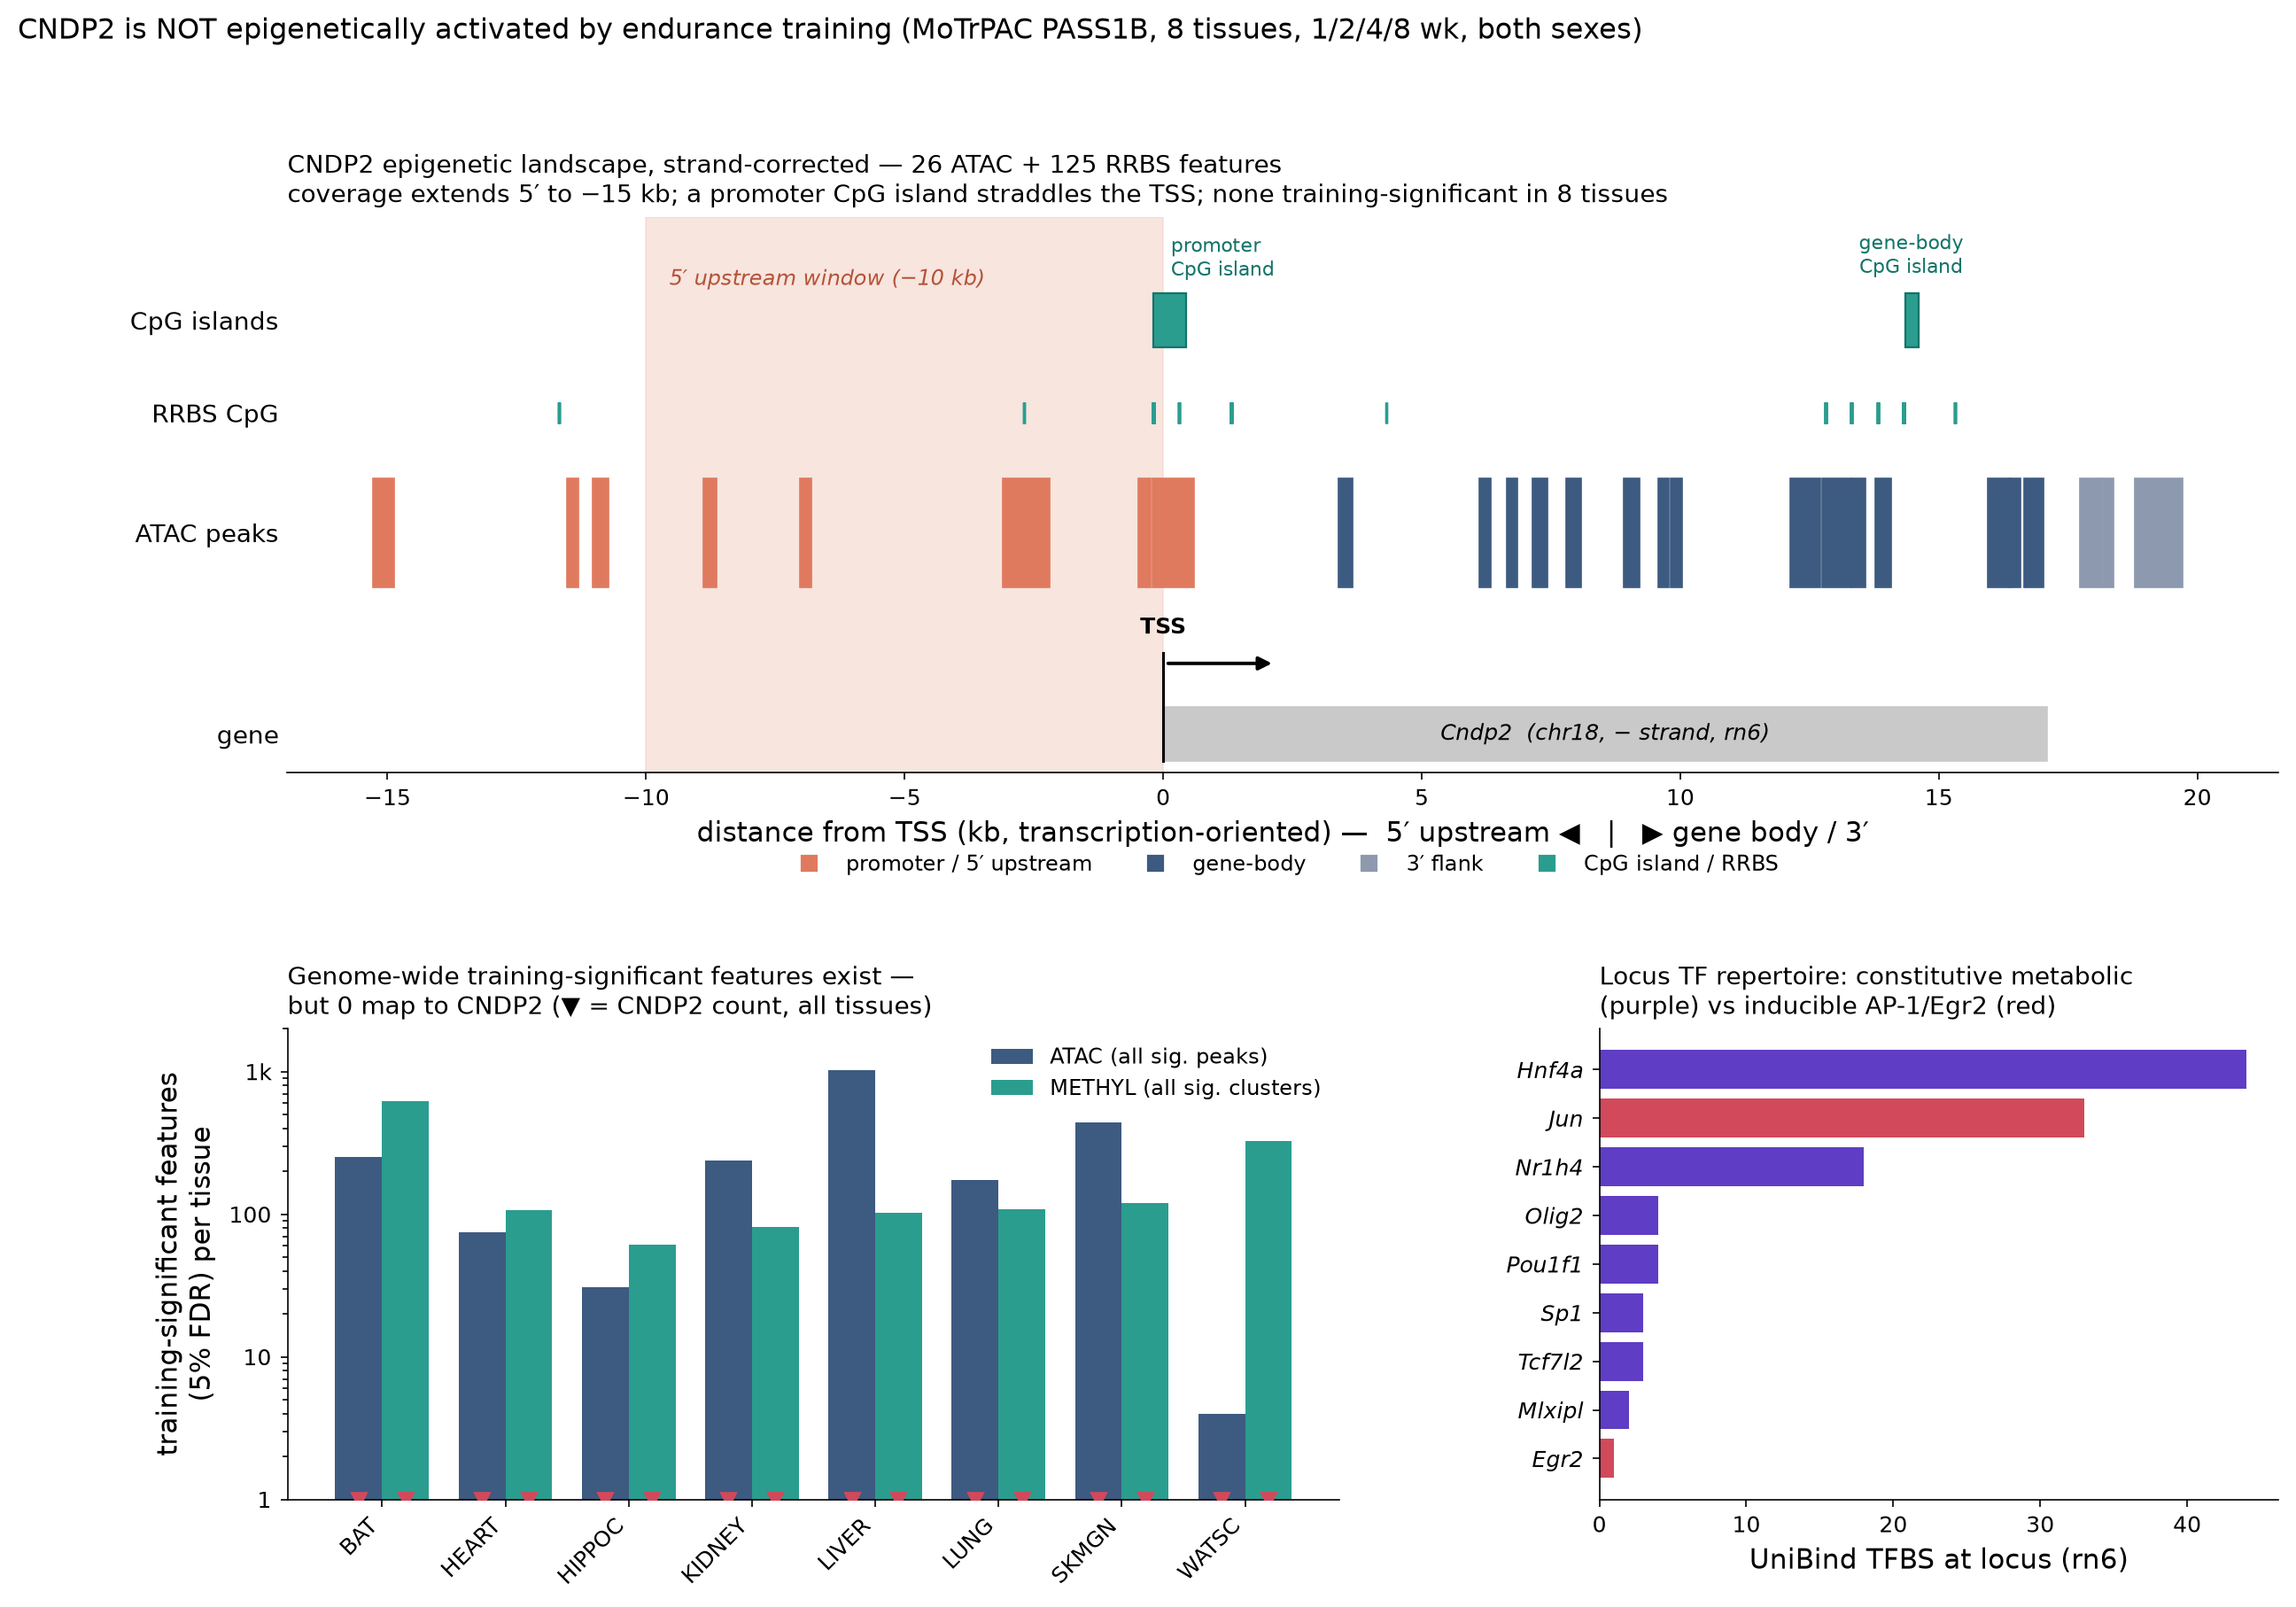
\includegraphics[width=\textwidth]{figures/figure4_cndp2_multiomic.png}\end{figure}

\textbf{Figure 5. CNDP2 shows no training-induced activation at any regulatory layer, including the promoter and 5$'$ upstream region.} \textit{Top: the strand-corrected CNDP2 epigenetic landscape. CNDP2 is a minus-strand gene (chr18, rn6); the axis is transcription-oriented, with the 5$'$ promoter/upstream region left of the TSS and the gene body/3$'$ end to the right. The 26 ATAC peaks (coloured by strand-corrected region) and 125 RRBS clusters are shown at their true positions: coverage extends 5$'$ to $\approx$$-$15 kb, and a promoter CpG island (chr18:81,538,627--81,539,249) straddles the TSS, with a second CpG island in the gene body. None of the 151 features is training-significant in any of 8 tissues, at any timepoint, in either sex; the same tissues carry hundreds-to-thousands of significant features genome-wide, of which 0 map to CNDP2. The locus TF repertoire is constitutive-metabolic (Hnf4a, Nr1h4/FXR, Mlxipl/ChREBP, Tcf7l2, Sp1) with only AP-1/Jun and a single Egr2 site inducible. Bottom: CNDP2 total protein is flat in 6 of 7 tissues but significantly decreased in liver (selection-aware FDR 0.012); phosphosites show only scattered nominal changes; the two most-regulated PTM sites are adjacent C-terminal lysines (acetyl-K364 significantly decreasing in liver, selection-aware FDR 0.018; ubiquityl-K363 increasing in liver, male-only, not selection-aware significant). The two significant liver effects are both decreases --- neither supports catalytic activation.}

\subsection*{2.4 CNDP2 protein and post-translational modifications show no activation}

The protein and PTM layers are also inconsistent with activation, though not uniformly
null (Figure 5, bottom). CNDP2 total protein is flat in 6 of 7 proteomics tissues (all

\textit{decreased}** (selection-aware FDR 0.012, both sexes, all timepoints; log\textsubscript{2}FC $-$0.06 to
$-$0.20) --- a direction opposite to activation. This extends the prior transcript- and
protein-abundance analysis, which had not flagged the liver decrease as significant, to
include white adipose (flat) and to report the liver result at its correct
significance. Among post-translational modifications, no site shows an increase
consistent with catalytic activation. The two most-regulated sites run the wrong way:
*\textit{acetyl-K364 is significantly }decreased*** in liver (selection-aware FDR 0.018, both
sexes; log\textsubscript{2}FC $-$0.14 to $-$0.41), and the only increasing signal --- ubiquityl-K363 in liver
--- is male-only, liver-only, and does not survive selection-aware correction (occupancy-normalised omnibus
p $\approx$ 3$\times$10\textsuperscript{$-$}\textsuperscript{3}; raw per-timepoint p $\approx$ 5$\times$10\textsuperscript{$-$}\textsuperscript{3}). Phosphosites (S58, S87, S299) show only scattered nominal changes, none
surviving correction.

Two liver layers --- total protein and acetyl-K364 --- are therefore statistically
significant, but both are \textit{decreases}, so neither supports a CNDP2-activation model; if
anything, hepatic CNDP2 is modestly down-regulated with training. No layer, in any
tissue, shows a training-associated \textit{increase} in CNDP2 abundance or an activating
modification.
Mapped onto CNDP2 structure (UniProt Q6Q0N1, an M20-family dinuclear metallopeptidase),
K363 and K364 are adjacent lysines in the C-terminal substrate-binding domain,
downstream of substrate-binding residues 330/343 and upstream of the metal-coordinating
residue 445 --- near, but not within, the catalytic machinery. Their proximity to that
domain makes them a plausible location for a modification that could modulate substrate
access, but the direction (a decrease) and the weak, non-generalising statistics do not
support an activation model.

Across all seven molecular layers, then --- transcript, chromatin accessibility, DNA
methylation, total protein, phosphorylation, ubiquitylation and acetylation --- CNDP2
carries no training-\textit{activation} signal (Table S1). The only significant training
effects are two hepatic \textit{decreases} (total protein and acetyl-K364), which point away
from, not toward, enzyme induction.

\textbf{Table 5. CNDP2 across all seven measured molecular layers.} No layer shows a training-associated \textit{increase}; the only two selection-aware-significant effects are hepatic \textit{decreases}.

{\footnotesize
\begin{longtable}{p{3.0cm}llp{2.6cm}p{3.4cm}}
\toprule
\textbf{Molecular layer} & \textbf{Assay coverage (tissues)} & \textbf{CNDP2 features} & \textbf{Training-significant} & \textbf{Direction / verdict} \\
\midrule\endhead
Transcript (RNA-seq) & 8 & 1 gene & none & flat (all tissues) \\
Chromatin access. (ATAC) & 8 & 26 peaks & 0 / 26 & no sig. peak, any tissue/tp/sex \\
DNA methylation (RRBS) & 8 & 125 clusters & 0 / 125 & no sig. cluster, any tissue/tp/sex \\
Total protein & 7 & 1 protein & LIVER down (sel-FDR 0.012) & DOWN in LIVER: log\textsubscript{2}FC -0.20 to -0.06 \\
Phosphorylation & 7 & S58/S87/S299 & none (selection-aware) & no sig. site \\
Ubiquitylation & 2 & K363 & none (selection-aware) & no sig. site \\
Acetylation & 2 & K364/K91 & LIVER down (sel-FDR 0.018) & DOWN in LIVER: log\textsubscript{2}FC -0.41 to -0.14 \\
\bottomrule
\end{longtable}
}



\subsection*{2.5 A modular in-silico pipeline de-risks hydrolysis-resistant Lac-Phe analogs before synthesis}

Because Lac-Phe production is substrate-driven rather than enzyme-gated, a therapeutic that
supplies the metabolite directly must overcome its central chemical liability: the
lactoyl--Phe amide bond is the site cleaved by peptidases and amidases, giving the native
molecule a short in-vivo residence that caps exposure regardless of dose. We therefore
assembled an in-silico panel of twelve Lac-Phe analogs (Figure 6a; Table 7) grouped by
mechanism. Three \textit{amide-retaining recognition blockers} keep the carbonyl but frustrate
enzymatic recognition --- \textit{N}-methylation removes the amide N--H required for the
peptidase hydrogen bond, an $\alpha$-methyl quaternary centre sterically shields the scissile
bond, and D-configuration defeats L-selective dipeptidases. Seven \textit{backbone
bioisosteres} replace the hydrolysable amide with a linkage that is not an amidase substrate:
some remove the amide carbonyl outright (a reduced amide/methyleneamine, a 1,2,3-triazole, and
(E)-alkene and (E)-fluoroalkene surrogates), while a thioamide (C=O$\rightarrow$C=S) and an
\textit{N}-acylsulfonamide retain the acyl carbonyl but replace the cleavable C--N bond, and a
ketomethylene removes the amide nitrogen. A \textit{retro-inverso} variant reverses bond
directionality. All twelve SMILES were validated with RDKit and their
physicochemical/druglikeness properties computed (molecular weight, cLogP by the Crippen
method, topological polar surface area, hydrogen-bond donors/acceptors, rotatable bonds and
QED; Figure 6b, Table 7). Every candidate passes the Lipinski rule-of-five and Veber rules
with zero violations, and --- apart from the more polar \textit{N}-acylsulfonamide --- sits
within the polar-surface-area window heuristically associated with CNS penetration, consistent
with the parent's central site of action on hypothalamic AgRP neurons via K\textsubscript{ATP}
channels [Liu 2025]. A PubChem record exists for the parent (CID 11075454, CAS 183241-73-8);
ChEMBL holds no Lac-Phe entry and no close structural analog, so no experimental bioactivity or
ADMET measurements are available. These are design candidates and computed property
predictions only --- none has been synthesized or assayed, and the upstream receptor that
senses Lac-Phe remains unidentified --- but they make concrete the persistence-engineering
strategy that the substrate-driven mechanism implies (Discussion 3.3).

We then ran the seven most tractable members --- the parent plus three amide-retaining
blockers ($N$-methyl, $\alpha$-methyl-Phe, D-Phe) and three carbonyl-modifying isosteres
(reduced amide, thioamide, 1,2,3-triazole) --- through a modular computational pipeline
that stages the questions a candidate must answer before it is worth making: will the bond
survive (stability), will it still be recognised (pharmacophore), will it be safe and
drug-like (ADMET), and does it bind like the parent (docking). These four CPU stages, run
from open data and making no assumption about the (still-unidentified) receptor, set the
composite ranking; a fifth stage --- physics-based Boltz-2 co-folding against the two
prioritized receptor pockets --- was then run on the shortlist as orthogonal structural
corroboration of the leads (Figure 7). \textbf{(i) Hydrolytic stability.} Semi-empirical
quantum chemistry (GFN2-xTB, implicit water) on the scissile linkage confirmed the design
premise: the carbonyl-free isosteres are inert by class --- the 1,2,3-triazole (aromatic, no
electrophilic carbon) and the reduced amide (sp$^3$ C--N) present nothing for water or a
peptidase to attack --- while the thioamide is only partially stabilised and the
amide-retaining blockers leave a cleavable bond. \textbf{(ii) Pharmacophore fidelity.} O3A
alignment to the parent scored preservation of the three SAR-relevant groups (terminal
carboxylate, lactoyl hydroxyl, amide H-bond vectors); $\alpha$-methyl-Phe gave the best raw
overlay but was penalised because $\alpha$-methylation is a known affinity-killer at
amino-acid-sensing receptors, making the overlay a geometric artefact. \textbf{(iii) ADMET.}
ADMET-AI (104 endpoints) returned uniformly clean hERG/CYP/AMES profiles and a shared, low
passive permeability intrinsic to the polar zwitterion (not rescued by any modification); the
one differentiating liability was a predicted drug-induced-liver-injury probability of 0.74 for
the triazole --- the highest in the panel, against 0.35--0.42 for the amide-retaining analogs and 0.14 for the reduced amide. All seven are
synthetically accessible (Ertl SAscore 2.4--3.1). \textbf{(iv) Candidate-target docking.}
Because the receptor is unknown, docking (smina) was scored on \textit{consistency with the
parent's binding mode} across a curated ten-receptor candidate panel rather than on raw
cross-chemotype energies (Discussion 3.3). \textbf{(v) Physics-based co-fold confirmation.} We then
co-folded the survivors against the two prioritized hydroxycarboxylic-acid-family pockets with
Boltz-2, scoring both a predicted affinity and a binder probability (Figure 7). Every ligand is
predicted to prefer HCAR1 (GPR81) over MRGPRD, and the two lead designs behave as the earlier
stages implied: the reduced amide (binder probability 0.73) and the 1,2,3-triazole (0.58) match or
exceed the parent (0.55), while the thioamide falls below it (0.39). Independent docking recovers the
parent's binding mode --- the same Arg94 salt-bridge and His256 $\pi$-stack at HCAR1 --- for
D-Phe, thioamide, triazole and reduced amide at sub-\r{a}ngstr\"om pose agreement, so the isosteres
that preserve the anionic carboxylate also preserve the interaction that anchors it. These results
enter the analysis as orthogonal structural corroboration of the two backbone-bioisostere leads; the
composite ranking (Table 8; 0.45$\cdot$stability + 0.40$\cdot$activity-retention
+ 0.15$\cdot$ADMET) nominates the \textbf{1,2,3-triazole} as lead --- the only design that makes
amide hydrolysis structurally impossible while preserving the load-bearing anionic carboxylate
--- with the reduced amide (cleanest ADMET, weaker pharmacophore match) and thioamide (most
shape-conservative) as backups. Critically, the same pipeline that nominates the triazole also
isolates its one liability --- a predicted drug-induced-liver-injury probability of 0.74, roughly
twice the next-highest analog (0.42) --- before a single compound is synthesised, so the lead is advanced
with its principal ADMET risk already named and prioritised for early experimental check. This
is computational prioritisation, not validation: the decisive experiments remain wet-lab
(serum/CNDP2 hydrolytic half-life, a receptor assay once a target is confirmed, and the in-vivo
anorectic readout).

\begin{figure}[H]\centering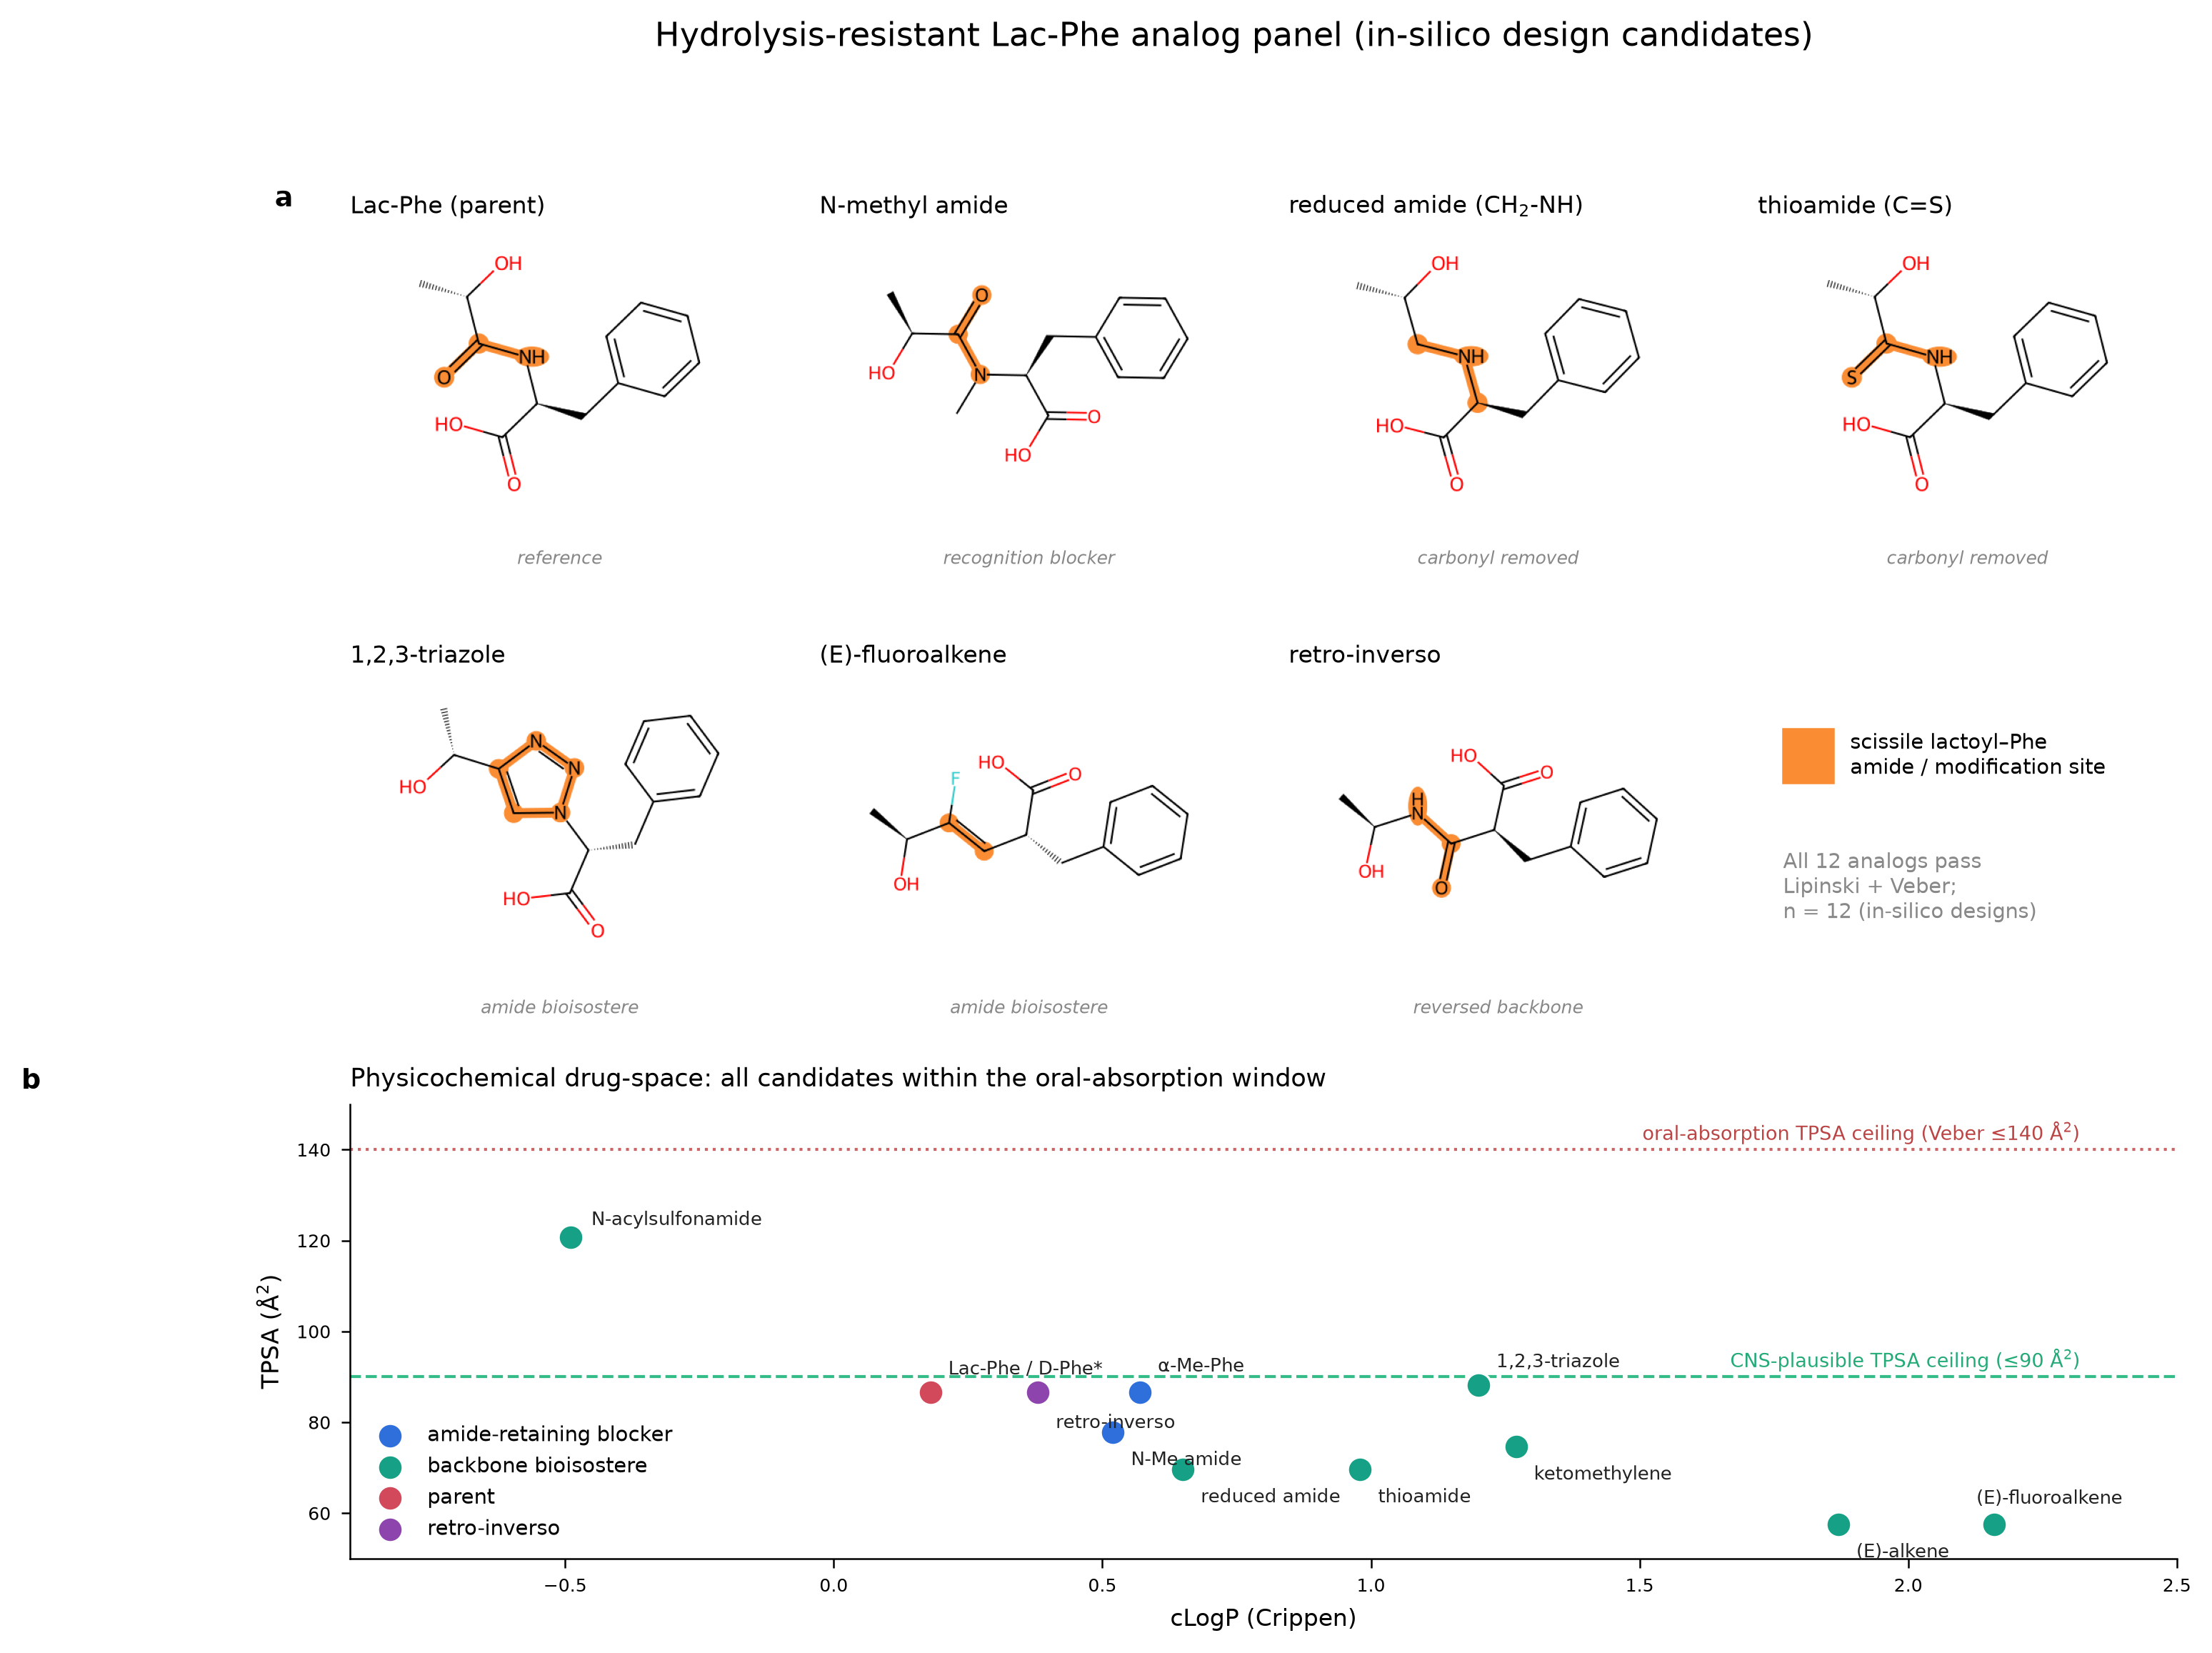
\includegraphics[width=\textwidth]{figures/figure5_drug_design.png}\end{figure}

\textbf{Figure 6. A hydrolysis-resistant Lac-Phe analog panel as candidate exercise-mimetic scaffolds (in-silico design).} \textit{(a) Parent Lac-Phe and representative analogs, one per mechanistic strategy; the scissile lactoyl--Phe amide (or the atoms replacing it) is highlighted in orange. (b) Computed physicochemical drug-space (cLogP versus TPSA) for all twelve panel members, coloured by mechanistic class; the Veber oral-absorption ceiling ($\leq$140 \r{A}$^2$, dotted) and the $\approx$90 \r{A}$^2$ CNS-penetration heuristic (dashed) are marked. All twelve pass Lipinski and Veber with zero violations. Properties are RDKit-computed (Crippen cLogP); values are predictions for design candidates that have not been synthesized or assayed. Lac-Phe (parent) and its D-Phe epimer share identical 2-D descriptors and overplot.}

\begin{figure}[H]\centering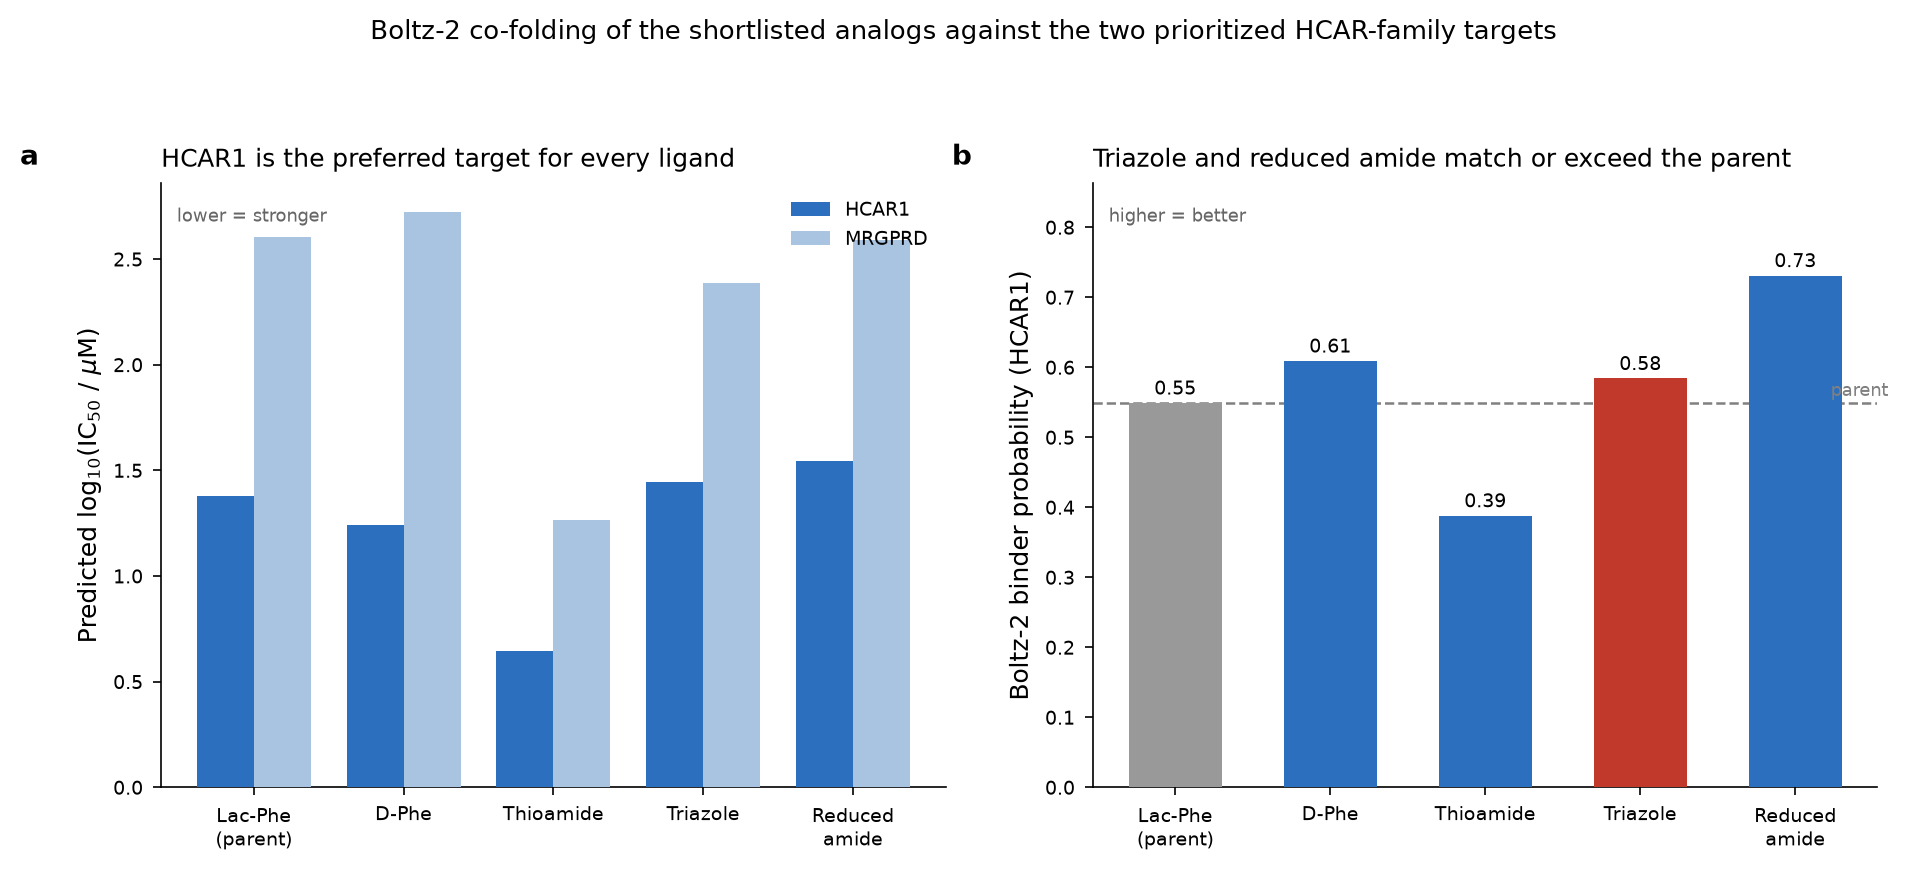
\includegraphics[width=0.95\textwidth]{figures/figure7_boltz_cofold.png}\end{figure}

\noindent\textbf{Figure 7. Boltz-2 co-folding of the shortlisted analogs against the two prioritized HCAR-family targets.} \textit{Physics-based co-fold and affinity-head predictions (Boltz-2) for the parent and four backbone survivors against HCAR1 (GPR81) and MRGPRD. (a) Predicted log\textsubscript{10} IC\textsubscript{50}: every ligand is predicted to bind HCAR1 more strongly than MRGPRD. (b) HCAR1 binder probability: the reduced amide (0.73) and the 1,2,3-triazole (0.58) match or exceed the parent Lac-Phe (0.55, dashed), while the thioamide (0.39) falls below it. Independent docking (shortlist not shown) reproduces the parent's Arg94 salt-bridge and His256 $\pi$-stack for D-Phe, thioamide, triazole and reduced amide at HCAR1 (pose agreement $\leq$0.7 \r{A}). These are computational binding predictions against a prioritized but still-unconfirmed receptor, not a validated affinity; they corroborate the two lead designs' mode of engagement rather than establish potency.}

\textbf{Table 7. Computed properties of the hydrolysis-resistant Lac-Phe analog panel (in-silico designs).} MW, molecular weight; cLogP, Crippen partition coefficient; TPSA, topological polar surface area (\r{A}$^2$); HBD/HBA, hydrogen-bond donors/acceptors; RotB, rotatable bonds; QED, quantitative estimate of druglikeness; L/V, Lipinski/Veber pass. Full descriptor set (fraction Csp$^3$, aromatic rings, BBB flag, database records) in \texttt{lacphe\_analogs\_admet.csv}.

{\footnotesize
\begin{longtable}{llrrrrrrrl}
\toprule
\textbf{Compound} & \textbf{Class} & \textbf{MW} & \textbf{cLogP} & \textbf{TPSA} & \textbf{HBD} & \textbf{HBA} & \textbf{RotB} & \textbf{QED} & \textbf{L/V} \\
\midrule\endhead
Lac-Phe (parent) & parent & 237.3 & 0.18 & 86.6 & 3 & 3 & 5 & 0.68 & yes/yes \\
N-Me amide & amide-retaining & 251.3 & 0.52 & 77.8 & 2 & 3 & 5 & 0.80 & yes/yes \\
alpha-Me-Phe & amide-retaining & 251.3 & 0.57 & 86.6 & 3 & 3 & 5 & 0.71 & yes/yes \\
D-Phe & amide-retaining & 237.3 & 0.18 & 86.6 & 3 & 3 & 5 & 0.68 & yes/yes \\
Reduced amide (CH2-NH) & backbone bioisostere & 223.3 & 0.65 & 69.6 & 3 & 3 & 6 & 0.66 & yes/yes \\
Thioamide (C=S) & backbone bioisostere & 253.3 & 0.98 & 69.6 & 3 & 3 & 5 & 0.68 & yes/yes \\
1,2,3-triazole & backbone bioisostere & 261.3 & 1.20 & 88.2 & 2 & 4 & 5 & 0.84 & yes/yes \\
N-acylsulfonamide & backbone bioisostere & 301.3 & -0.49 & 120.8 & 3 & 5 & 6 & 0.65 & yes/yes \\
Ketomethylene & backbone bioisostere & 236.3 & 1.27 & 74.6 & 2 & 3 & 6 & 0.78 & yes/yes \\
(E)-alkene & backbone bioisostere & 220.3 & 1.87 & 57.5 & 2 & 2 & 5 & 0.74 & yes/yes \\
(E)-fluoroalkene & backbone bioisostere & 238.3 & 2.16 & 57.5 & 2 & 2 & 5 & 0.83 & yes/yes \\
Retro-inverso & retro-inverso & 237.3 & 0.38 & 86.6 & 3 & 3 & 5 & 0.51 & yes/yes \\
\bottomrule
\end{longtable}
}



\textbf{Table 8. Ranked decision matrix for the seven-member triage panel.} Composite = 0.45$\cdot$hydrolytic-stability + 0.40$\cdot$activity-retention + 0.15$\cdot$ADMET-factor; activity-retention blends pharmacophore fidelity and parent-consistent docking and applies the $\alpha$-methyl-Phe recognition penalty. DILI, predicted drug-induced-liver-injury probability; Co-fold P, Boltz-2 predicted HCAR1 binder probability (Figure 7; --- = not co-folded), reported alongside but not folded into the composite; SAscore, Ertl synthetic-accessibility. Stages and full axes in \texttt{Lac-Phe\_analog\_report.md} and \texttt{decision\_matrix.csv}. $^\dagger$The triazole DILI flag is the one liability to verify experimentally.

{\footnotesize\setlength{\tabcolsep}{4pt}
\begin{longtable}{llccccccl}
\toprule
\textbf{Rank} & \textbf{Analog} & \textbf{Composite} & \textbf{Stability} & \textbf{Activity ret.} & \textbf{DILI} & \textbf{Co-fold P} & \textbf{SAscore} & \textbf{Route} \\
\midrule\endhead
--- & Lac-Phe (parent) & 0.59 & 0.10 & 1.00 & 0.32 & 0.55 & 2.44 & amide coupling \\
\textbf{1} & \textbf{1,2,3-triazole} & \textbf{0.87} & \textbf{1.00} & \textbf{0.80} & \textbf{0.74$^\dagger$} & \textbf{0.58} & \textbf{3.05} & \textbf{CuAAC} \\
2 & Reduced amide & 0.80 & 0.95 & 0.56 & 0.14 & 0.73 & 2.52 & red. amination \\
3 & Thioamide & 0.70 & 0.60 & 0.71 & 0.36 & 0.39 & 2.88 & Lawesson \\
4 & N-Me amide & 0.55 & 0.35 & 0.63 & 0.42 & --- & 2.81 & amide coupling \\
5 & D-Phe & 0.54 & 0.15 & 0.81 & 0.35 & 0.61 & 2.44 & amide coupling \\
6 & alpha-Me-Phe & 0.45 & 0.35 & 0.37 & 0.38 & --- & 2.87 & amide coupling \\
\bottomrule
\end{longtable}
}

\section*{3. Discussion}

Two questions have shadowed Lac-Phe since its discovery, and prior analyses of exercise
atlases have tended to answer them as one. The first is whether the metabolite is present
and training-responsive in a given tissue; the second is \textit{why} --- whether a training
response, where it exists, reflects induction of the enzyme that makes Lac-Phe or simply a
change in the substrate handed to a constitutive enzyme. By returning to the raw MoTrPAC
spectra we can address both in the single most comprehensive exercise dataset assembled to
date, and the two answers point the same way: an ion at Lac-Phe's exact mass is detectable
across all 19 PASS1B tissues (1,380 biological samples), its training response is transient
and tissue-restricted --- robust only in the heart, and only on the selection-free omnibus
(q = 0.014) --- and CNDP2 itself is not activated at any of the seven molecular layers
MoTrPAC measures. Read together, these say that Lac-Phe behaves as a substrate-driven
metabolite whose output tracks flux, not enzyme dosage. The sections below develop that
reading, place it against the organ-level biology now emerging from the primary literature,
and state --- within tightly bounded confidence --- what it implies for turning an
exercise metabolite into a drug.

\subsection*{3.1 A substrate-driven metabolite, read correctly, predicts a flat enzyme}

The convergent negative at CNDP2 is the paper's central mechanistic result, and it is best
read not as a puzzle but as a confirmation. The founding biochemistry frames Lac-Phe
production as substrate-limited rather than enzyme-limited: N-lactoyl amino acids are formed
by CNDP2 running in reverse, a reverse-proteolysis reaction whose product tracks the
mass-action availability of lactate and the free amino acid rather than the amount of enzyme
present [Jansen 2015]. That framing carries a built-in prediction, and the human genetics
of phenylketonuria supplies the cleanest test of it: when phenylalanine is chronically
elevated, Lac-Phe rises in proportion, with no implied change in CNDP2 [Jansen 2015]. The
two interventions that most raise Lac-Phe elsewhere behave the same way --- intense exercise
and metformin both act by raising \textit{lactate}, not CNDP2 protein [Xiao 2024a; Scott 2024;
Li 2023], and the founding study reports that the pre-versus-post-exercise fold-change of
Lac-Phe correlates with that of lactate at r = 0.82 (p $<$ 0.0001) in humans [Li 2022]. If
flux is set by substrate, the metabolite can swing widely while the enzyme stays flat, or
even falls.

Our seven-layer result is exactly that signature. Across chromatin accessibility, DNA
methylation, transcript, total protein, and phospho-, ubiquityl- and acetyl-modifications,
no layer shows a training-associated \textit{increase} at the CNDP2 locus in any assayed tissue;
of 151 epigenetic features (26 ATAC peaks, 125 methylation clusters) none reaches
significance in any of 8 tissues, and the only two significant effects anywhere --- hepatic
total protein and acetyl-K364 --- are \textit{decreases}. This is not an assay-sensitivity artifact:
the same tissues carry thousands of training-significant epigenetic features genome-wide,
and the heart, the one tissue where the metabolite signal is statistically robust, itself
carries 75 significant ATAC peaks and 107 significant methylation clusters --- none at CNDP2.
The result therefore rules out, at every layer MoTrPAC measures, the most obvious
alternative to a substrate-driven model: that the metabolite response is a readout of enzyme
induction. The locus annotation sharpens the point. The CNDP2 promoter and gene body are
dominated by constitutive hepatic/renal metabolic transcription factors (Hnf4a, the
bile-acid receptor Nr1h4/FXR, Mlxipl/ChREBP, Tcf7l2, Sp1), with only AP-1/Jun and a single
Egr2 site representing the activity-inducible repertoire --- the wiring of a housekeeping
conjugase, not of an exercise-inducible effector gene.

This places Lac-Phe in an instructive position within the exerkine landscape. Many mediators
of the exercise response are induced factors --- secreted proteins and peptides whose
transcription or release rises with training [Chow 2022] --- and it would have been reasonable
to expect a metabolite messenger to be governed the same way, through the abundance of its
maker. Lac-Phe is not: it belongs with the class of exercise signals set by metabolic flux,
of which lactate itself is the archetype [Brooks 2023]. The distinction is not semantic. It
is precisely why "substrate, not switch" is the correct verb for this system, and why a
snapshot of enzyme abundance --- the readout most atlases would reach for --- is the wrong
instrument to detect a Lac-Phe response. We are careful not to over-read the mechanism from
a single cross-sectional atlas: the enzyme-flat result bounds the \textit{direction} of regulation,
not the absolute flux, and identity here rests at MSI Level 2. But the direction is
unambiguous, and it is the direction the founding biochemistry predicts.

\subsection*{3.2 An organ source--sink model explains the time courses}

Placing the cross-tissue data against the primary literature yields a coherent organ-level
picture (Figure 1b). Lac-Phe is a blood-borne metabolite with distributed synthesis and
specialised clearance. It is made wherever CNDP2 meets lactate and phenylalanine ---
principally the intestinal epithelium at rest and after metformin [Xiao 2024a; TeSlaa 2024;
Ghias 2025], and contracting skeletal muscle and its resident immune cells during exercise
[Li 2022; Everaert 2012] --- exported to a common plasma pool, and excreted by the kidney
through the SLC17A1/3 transporters, which decouple the urine pool from the blood pool such
that transporter knockout lowers urine but not plasma Lac-Phe [Li 2024]. In PASS1B kidney,
neither \textit{Slc17a1} nor \textit{Slc17a3} is training-regulated at transcript or protein
(all training contrasts non-significant), so renal clearance capacity is a constitutive term:
the plasma pool is set by production, not by induced transport, which is consistent with
kidney reading as a training-associated \textit{decrease} (clearance of a rising pool) rather
than a source. The brain is where
the circulating signal \textit{acts}, directly inhibiting hypothalamic AgRP neurons via
K\textsubscript{ATP}-channel activation to drive hypophagia [Liu 2025] --- a receptor/effector site rather
than a large metabolic pool. Adipose is positioned as a downstream responder whose
remodeling the circulating signal predicts, the pivotal human observation being that
post-exercise plasma Lac-Phe forecasts abdominal adipose loss over an endurance program
[Hoene 2022].

This model accounts for each feature of our data, and does so quantitatively where the
literature allows. Ubiquitous detectability follows directly from a circulating analyte
distributed to every perfused tissue: the shared plasma pool guarantees a measurable ion in
all 19 tissues without requiring autonomous local production. A tissue-restricted training
\textit{effect}, by contrast, requires a compartment where local substrate flux changes enough to
lift the local pool above that plasma background. The heart is the strongest candidate on
first principles --- continuously perfused, an avid lactate consumer, and subject to a
sustained workload increase with training --- and it is precisely the tissue where the effect
survives the selection-free omnibus (q = 0.014), with plasma and white adipose concordant
across ionization modes but suggestive only. This is not merely a post-hoc rationalisation
of which tissue "won": an orthogonal multi-tissue integration of the same PASS1B animals
places heart within a tightly coupled visceral/secretory organ module (heart--kidney,
heart--liver, heart--lung all co-varying within individual animals after the shared training
timeline is removed) whose members are the high-perfusion, high-substrate-flux organs the
source--sink model flags as most tightly coupled to the circulating pool. The compartment
first-principles nominate as the Lac-Phe integrator is the same one an unsupervised
cross-tissue analysis identifies as a coordinated metabolic hub.

The transient time course follows from mass action under training adaptation. Endurance
training lowers the blood-lactate response to a fixed workload, so a substrate-driven signal
is largest early --- in na\"\i{}ve animals, at high relative intensity and high lactate --- and
shrinks as the lactate response adapts; read across a cross-sectional weeks-1/2/4/8 design,
that is an early rise decaying by week 8. The human data are consistent on both the acute
and the chronic limb: circulating Lac-Phe scales with exercise intensity in a randomized
crossover trial, tracking the lactate load [Weber 2025], and within-subject longitudinal
sampling shows the acute per-session rise attenuating numerically over a training program,
albeit as a non-significant trend in an exploratory cohort [Glatz 2025]. The female
predominance is a robust feature of our multi-tissue data that prior work has largely not been
positioned to see: sex-specific Lac-Phe dynamics are reported acutely in one human study
[Bauhaus 2025], while most N-lactoyl-amino-acid work is single-sex or does not analyse sex. The
substrate/clearance framework accommodates it directly --- sex differences in phenylalanine
availability, in the relative-intensity lactate response at matched absolute workload, or in
renal clearance all sit upstream of CNDP2 --- and it is a specific, testable prediction for
sex-resolved follow-up.

A design feature of the atlas sharpens this reading. PASS1B collected every tissue
$\approx$48 h after the last exercise bout, a deliberate washout that captures a
trained-recovered state rather than the acute post-exercise window in which plasma Lac-Phe
spikes most steeply [Li 2022]. For an acute, substrate-driven metabolite this timing predicts
exactly what we see --- most tissues flat, the surviving signal a modest chronic-adaptation
residual well below the acute excursion --- and it explains why the feature never rose above
MoTrPAC's peak-picking threshold in the first place: the atlas was, by design, sampling away
from Lac-Phe's peak.

Two structural caveats bound the model. The PASS1B design is cross-sectional, so "transient"
is an across-group inference, not a within-animal trajectory; the closest longitudinal
analogue, the within-subject attenuation reported by [Glatz 2025], is in humans and does not
reach significance. And much of the organ-role evidence --- gut source, kidney clearance, AgRP
site of action --- is from mouse genetic models assumed, but not here shown, to be conserved in
rat. The source--sink model is a framework for interpreting the time courses, not a claim
that each rat tissue has been directly assigned a source or sink role.

\subsection*{3.3 Implications for an exercise-mimetic}

Because this analysis confirms Lac-Phe's identity only to MSI Level 2 and does not establish
absolute concentrations, its therapeutic implications are stated as an explicitly speculative
argument, anchored wherever possible to real doses and validated pharmacology. The exogenous
intervention that produces the demonstrated anti-obesity effect is 50 mg/kg Lac-Phe i.p. in
diet-induced obese mice; notably, the same administration suppresses feeding in obese but not
lean mice even at 150 mg/kg --- an obesity-state specificity rather than a simple dose effect
[Li 2022]. The physiological stimulus this mimics is acute: sprint exercise produces the
largest human plasma Lac-Phe elevation, still detectable hours later [Li 2022], and intensity
sets the magnitude [Weber 2025]. Our training-induced changes are, by contrast, modest peak
fold-changes (plasma $\approx$ 1.4$\times$, heart $\approx$ 2.1$\times$, white adipose $\approx$ 2.4$\times$ versus sedentary) --- a
chronic-adaptation residual well below the acute post-exercise excursion, exactly as a
substrate-driven metabolite tracking the (adapting) lactate response should read in a
sustained-training cross-section.

The substrate-driven mechanism reframes what a Lac-Phe-raising exercise-mimetic must do. The
levers are not the enzyme. Raising CNDP2 expression is unlikely to help, since the enzyme is
not rate-limiting and is not induced even by real training; the tractable levers are
\textbf{substrate supply} and \textbf{molecular persistence}. A drug that raises the relevant lactate
microenvironment reproduces the physiological trigger --- which is mechanistically how
metformin already engages this axis [Xiao 2024a; Scott 2024] --- while direct administration of
Lac-Phe, or of a hydrolysis-resistant analog, bypasses synthesis entirely.

The persistence lever deserves more than the single clause it has previously been given,
because it has strong pharmacological precedent. Lac-Phe is a pseudodipeptide --- an
N-lactoyl amide --- and its central liability as a drug is the same one that governs peptide
messengers generally: the amide bond is a substrate for hydrolysis, giving a short
in-vivo residence that caps exposure regardless of how much is dosed. The medicinal-chemistry
response to that liability is mature. The canonical case is the incretin GLP-1, an endogenous
peptide whose native half-life is on the order of minutes because it is cleaved rapidly in
circulation [M\"uller 2019]; engineering a protease-resistant, albumin-binding analog converted
that transient signal into a once-weekly therapeutic (semaglutide), which is now among the
most effective anti-obesity drugs in use [Yang 2024]. The general toolkit for extending the
metabolic stability of small peptides and peptidomimetics --- backbone amide bioisosteres,
N-methylation, D-amino-acid and reduced-bond substitutions, and conjugation strategies --- is
well established [Yao 2018]. Applied to Lac-Phe, the target is narrower and arguably more
tractable than a full peptide: a single hydrolysis-prone amide, whose replacement by an
amide bioisostere that preserves recognition while resisting cleavage would convert the brief,
substrate-driven pulse the physiology delivers into the sustained exposure a drug requires.
This is the reading the transient kinetics force: pharmacokinetics --- turning a pulse into a
plateau --- will govern efficacy as much as peak level.

Two boundaries keep this speculation honest. First, the receptor that \textit{senses} Lac-Phe is
still unidentified. The downstream circuit is now defined --- Lac-Phe silences AgRP neurons
through K\textsubscript{ATP}-channel opening, with MC4R- and NPY1R-expressing paraventricular neurons
required for the full anorexigenic response [Liu 2025] --- but the upstream sensor that
transduces extracellular Lac-Phe into that K\textsubscript{ATP} response has not been found, and the GDF15
receptor GFRAL has been experimentally excluded [Xiao 2024a]. Our own target-agnostic docking
offers one mechanistically coherent \textit{hypothesis} to test rather than an answer: across a
ten-receptor candidate panel, the parent and its analogs most consistently reproduce a
carboxylate salt-bridge binding mode in the hydroxycarboxylic-acid receptor HCAR1 (GPR81, the
L-lactate receptor) --- an appealing candidate precisely because Lac-Phe is an acyl-lactate, so
a lactate-sensing GPCR is a natural first suspect. Physics-based Boltz-2 co-folding of the
shortlisted analogs (Figure 7) reinforces this ordering: every ligand is predicted to prefer
HCAR1 over the alternative MRGPRD pocket, and the co-fold recovers the parent's Arg94
salt-bridge and His256 $\pi$-stack for the backbone survivors --- structural corroboration that
the carboxylate-anchored pose is at least self-consistent. We stress that co-folding scores
pose plausibility and predicted binding, not measured affinity, and cannot by itself identify
the physiological sensor; HCAR1 is a prioritised deorphanization target, now with converging
in-silico support, not a confirmed receptor. Until the true sensor is confirmed, a receptor-agonist
mimetic cannot be designed rationally, which is itself an argument for the two levers above:
raising substrate flux and administering a persistence-engineered Lac-Phe (or analog) are the
paths that do not wait on deorphanization. Second, target engagement is
not the same as a therapeutic window. The obesity-state specificity of the anti-obesity
effect [Li 2022], and the emerging human association of N-lactoyl amino acids with insulin
resistance and diabetic complications [Naja 2025], together indicate that dose, exposure and
metabolic context --- not merely raising the metabolite --- will define where benefit turns to
liability; the completed intravenous Lac-Phe-versus-saline trial in overweight/obese adults
[NCT06743009] is the first direct human read on exactly that window. Lac-Phe thus sits within,
and is disciplined by, the broader exercise-mimetic search --- from betaine, recently nominated
as a geroprotective exercise mimetic through an unbiased screen [Geng 2025], to the exerkine
landscape more broadly [Chow 2022] --- as one defined, endogenous, and now mechanistically
constrained candidate among several.


\subsection*{3.4 Limitations}

Identity rests on accurate mass, retention time, and four converging MS1 lines of evidence,
supported by an in-silico fragmentation that matches the observed in-source ions; the
MoTrPAC deposit contains no acquired MS/MS and Lac-Phe is absent from public spectral
libraries, so Level-1 confirmation requires an authentic-standard co-injection that no public
dataset can provide. The in-source fragment ions are shared with co-eluting free
phenylalanine, so they corroborate the assignment only through their per-sample covariation
with the intact ion, not as unique Lac-Phe signatures. The training-response inference is
honest but narrow: only the heart signal is robust, and only on the selection-free omnibus
(q = 0.014); no tissue survives the stricter selection-aware correction, so even the heart
result is best held as strong-but-provisional, and the plasma and white-adipose transients as
hypothesis-generating. The CNDP2-activation analysis is bounded by what MoTrPAC assayed --- the
significance-filtered epigenetic objects report only whether CNDP2 crosses threshold, not its
sub-threshold effect size; PTM coverage is uneven (ubiquitylation and acetylation only in
heart and liver); and all inference is at the level of a picked chromatographic peak, without
absolute quantitation. These bound the strength, not the direction, of the conclusions: the
convergent absence of any activating change, against tissues that carry thousands of
training-responsive features, is a positive result about how Lac-Phe is regulated, even as
the metabolite's precise level in each tissue remains for standard-confirmed, MS/MS-enabled
follow-up.

\section*{4. Methods}

\textbf{Raw-spectra extraction.} For each Metabolomics Workbench study we read the ZIP64
central directory of the raw-data archive over HTTP range requests and extracted
individual per-sample acquisitions without downloading the whole multi-GB archive.
Agilent centroided spectra (\texttt{MSPeak.bin}) were decoded scan-by-scan, retaining only
peaks within 10 ppm of the target m/z. The ten HILIC-only tissues, stored in the
x86-64-only Thermo \texttt{.raw} format, were converted to mzML with ThermoRawFileParser in a
Linux container and processed identically. Extracted-ion chromatograms were integrated
at a consensus apex within the validated retention window. The extraction pipeline is
released as a reproducible skill with a full 28-study/19-tissue manifest.

\textbf{Compute orchestration.} The analysis ran on a deliberately heterogeneous stack matched
to the data. All Agilent \texttt{.d} extraction, extracted-ion-chromatogram integration, and the
full statistical workload (per-week Mann--Whitney, selection-free Kruskal--Wallis omnibus,
selection-aware permutation nulls, and the 28-study FDR control) ran locally on a macOS
workstation (14 CPU cores, no discrete GPU). Only the step that could not run locally --- reading
the x86-64-only Thermo \texttt{.raw} vendor format --- was offloaded to ephemeral Modal Linux
containers running ThermoRawFileParser, which returned open-format mzML for identical local
processing. Rather than download the multi-gigabyte per-study archives, we parsed each archive's
ZIP64 central directory and pulled only the byte ranges of the individual acquisitions needed over
HTTP range requests, keeping network transfer to a small fraction of the deposited volume. The
whole pipeline --- remote vendor-format conversion, range-request extraction, and permutation
testing --- was orchestrated end-to-end by an agentic analysis system (Claude Science), which also
performed the literature verification below.

\textbf{Positive-control validation.} To verify the bespoke extraction quantitatively, twelve
metabolites present in MoTrPAC's released plasma reversed-phase-negative table (ST002632),
spanning the retention-time and abundance range, were extracted from the same 50
biological raw files with the identical pipeline and integrated at their consensus apex.
Per-sample log\textsubscript{2} abundances were compared to the released named-metabolite matrix by
Pearson correlation; per-week $\Delta$log\textsubscript{2}FC (each training week vs the balanced sedentary
control) was compared to the released dose-response. Mass accuracy (median ppm) and
retention-time agreement were computed against the released m/z and RT
(Table 1, Figure 4).

\textbf{Statistics.} Because MoTrPAC responses are frequently non-monotonic, each feature was
tested per timepoint (Mann-Whitney versus sedentary), with a Kruskal-Wallis timecourse
omnibus, and sex-stratified. Every tissue was held to two complementary bars. The \textit{selection-free} bar is the
Kruskal--Wallis timecourse omnibus, which evaluates weeks 0/1/2/4/8 jointly and makes no
choice of a peak week. The \textit{selection-aware} bar takes the natural peak-week effect
statistic --- the maximum weekly $\Delta$log\textsubscript{2} increase per study --- and controls it
against a 5,000$\times$ week-label permutation null that recomputes the same best-week statistic,
so that a surviving signal is robust to peak-week selection; a decoy panel of 64 m/z bounds the
false-positive rate. Both were FDR-corrected across studies. Reporting against both bars, rather
than a single threshold, is what licenses the confident single-responder claim in the Results. Within each tissue and mode the per-sample matrix was balanced to the intended
5 animals/sex/week design over weeks 0/1/2/4/8 (reversed-phase 968$\rightarrow$888 rows;
HILIC 492 extracted$\rightarrow$420 analyzed), removing surplus QC/replicate injections. Undetected
samples were floored to the per-feature minimum, each tissue$\times$week$\times$sex cell was summarised by
its median, and trained-week cells were compared to the same-sex week-0 control by an
\textit{exact} Mann--Whitney test; the exact variant is load-bearing (the asymptotic
approximation shifts borderline p-values, e.g. heart-male week 2 from 0.15 to 0.12, without
changing the effect estimates). Peak $\Delta$log\textsubscript{2} magnitudes are pooled-sex per-sample
summaries at the peak week versus sedentary control and should be read as approximate; the
significance tests do not depend on the summary choice. Reported fold-changes are the corresponding
peak-week/control ratios.

\textbf{CNDP2 multi-omic analysis.} ATAC-seq and RRBS methylation
(\texttt{ATAC\_*/METHYL\_*\_NORM\_DATA\_05FDR} and the timewise differential set) and proteome,
phospho-, ubiquityl- and acetyl-proteome (\texttt{PROT\_*/PHOSPHO\_*/UBIQ\_*/ACETYL\_*\_DA} and
\texttt{NORM\_DATA}) objects were obtained from the MotrpacRatTraining6moData package. CNDP2
features were identified by Ensembl ENSRNOG00000015591 / RefSeq NP\_001010920.1 / gene
symbol Cndp2, mapped to the rat chromosome-18 locus, and tested with the same
timecourse/selection-aware framework. Phosphosite occupancy was normalised to total
protein where possible. The CNDP2 regulatory landscape was annotated with UniBind rat
TFBS and JASPAR matrices; PTM sites were mapped onto UniProt Q6Q0N1.

\textbf{Hydrolysis-resistant analog panel.} Twelve Lac-Phe analogs spanning three
mechanistic classes (amide-retaining recognition blockers; backbone amide bioisosteres;
retro-inverso) were specified as canonical SMILES and validated with RDKit
(\texttt{MolFromSmiles}). Physicochemical and druglikeness descriptors --- molecular weight,
Crippen cLogP, topological polar surface area, hydrogen-bond donors/acceptors, rotatable
bonds, aromatic-ring count, fraction Csp$^3$ and QED --- and Lipinski rule-of-five and Veber
compliance were computed with RDKit. Database records were queried for the parent and each
analog via PubChem and ChEMBL. Seven tractable members were then triaged through a
CPU funnel of four executed stages: hydrolytic-stability proxies from semi-empirical quantum
chemistry (GFN2-xTB, implicit water) on the scissile linkage; pharmacophore fidelity by RDKit
O3A alignment to the parent; ADMET across 104 endpoints (ADMET-AI) and Ertl synthetic
accessibility; and parent-consistency docking (smina) against a curated ten-receptor candidate
panel scored on reproduction of the parent's binding mode. Boltz-2 co-folding and affinity-head
scoring (Boltz-2, MSA-free single-sequence mode, one predicted complex per ligand--receptor pair)
were then run for the survivors against the two prioritized pockets (HCAR1/GPR81 and MRGPRD),
returning per-complex confidence/ipTM, a predicted affinity value (reported as log\textsubscript{10}
IC\textsubscript{50}) and a binary binder probability, together with a docked pose whose
salt-bridge and $\pi$-stack contacts were compared to the co-folded parent's (Figure 7); the
runnable bundle is released as \texttt{boltz\_local.tar.gz} and the scores as
\texttt{boltz\_affinity\_scores.csv}. The four
computational stages set the composite ranking; the co-fold enters as orthogonal structural
corroboration of the leads. A composite score
(0.45$\cdot$stability + 0.40$\cdot$activity-retention + 0.15$\cdot$ADMET) produced the ranked
matrix (Table 8; \texttt{decision\_matrix.csv}, with full per-stage methods and caveats in
\texttt{Lac-Phe\_analog\_report.md}). No compound was synthesized or experimentally assayed;
all reported values are computed predictions (Figures 6, Tables 7--8).

\textbf{Literature synthesis.} Primary sources were retrieved and each DOI verified against
its record (title, authors, venue, year) via OpenAlex and PubMed; 46 references passed verification, each DOI checked live against its record; two papers flagged as retracted were excluded.

\section*{Data and code availability}

Underlying data are MoTrPAC PASS1B, public on Metabolomics Workbench (studies ST002628--
ST002916) and in the MotrpacRatTraining6moData package. The raw-spectra extraction
pipeline is released as a reproducible skill. Supplementary Table S1
(\texttt{cndp2\_multiomic\_supplementary.xlsx}) gives per-assay/tissue/site statistics with strand-corrected CNDP2-locus coordinates; the
positive-control concordance (\texttt{pc\_concordance\_table.csv}) and the verified reference set
(\texttt{lacphe\_literature\_refs.csv}) are provided alongside; the analog campaign's ranked matrix (\texttt{decision\_matrix.csv}), full written report (\texttt{Lac-Phe\_analog\_report.md}) Boltz-2 co-fold bundle (\texttt{boltz\_local.tar.gz}) and co-fold affinity scores (\texttt{boltz\_affinity\_scores.csv}) accompany the drug-design section. In-text Tables 1--6 reproduce the
key rows of these files directly.

\textbf{Code availability.} All code to regenerate every figure, table, and the compiled PDF
from raw data --- the raw-spectra extraction pipeline, the positive-control benchmark, the
CNDP2 multi-omic analysis, the statistics, and the figure/table build scripts --- together
with a pinned environment file, a README giving exact run instructions (raw data $\rightarrow$
figures $\rightarrow$ compiled PDF), and an independent correctness audit of this manuscript, is
provided as a reproducibility package at \url{https://github.com/USERNAME/REPO}
(placeholder --- the repository is assembled and runs from a clean checkout; the public URL
will be inserted on deposit).


\textbf{Table 6. Reference-verification sample (10 of the 44 Lac-Phe and context literature sources; every DOI checked live against its record).} All resolve with no retractions; the full set with per-source claims is in \texttt{lacphe\_literature\_refs.csv}. The reference list totals 46 entries: 44 Lac-Phe, exercise-physiology, and drug-design sources plus two MoTrPAC consortium method references (Amar 2024, Schenk 2024; refs 45--46).

\begin{longtable}{llll}
\toprule
\textbf{First author, year} & \textbf{Venue} & \textbf{DOI} & \textbf{Verified} \\
\midrule\endhead
Jansen 2015 & Proceedings of the Nat & 10.1073/pnas.1424638112 & \checkmark \\
Hoene 2022 & Metabolites & 10.3390/metabo13010015 & \checkmark \\
Li 2022 & Nature & 10.1038/s41586-022-04828-5 & \checkmark \\
Moya-Garzon 2024 & Cell & 10.1016/j.cell.2024.10.032 & \checkmark \\
Li 2024 & Nature communications & 10.1038/s41467-024-51174-3 & \checkmark \\
Xiao 2024 & Nature metabolism & 10.1038/s42255-024-00999-9 & \checkmark \\
Scott 2024 & Nature metabolism & 10.1038/s42255-024-01018-7 & \checkmark \\
Liu 2025 & Nature metabolism & 10.1038/s42255-025-01377-9 & \checkmark \\
Ghias 2025 & American journal of ph & 10.1152/ajpendo.00037.2025 & \checkmark \\
Glatz 2025 & Diabetes, obesity \& me & 10.1111/dom.70236 & \checkmark \\
\bottomrule
\end{longtable}

\section*{References}

\begin{enumerate}
\item Otani H, et al. (2008). \textit{Neurosci Lett}. https://doi.org/10.1016/j.neulet.2008.09.008 --- CNDP2 tissue dipeptidase characterisation.
\item Everaert I, et al. (2012). \textit{Eur J Appl Physiol}. https://doi.org/10.1007/s00421-012-2540-4 --- CNDP2 in human skeletal muscle.
\item Oku N, et al. (2012). \textit{Biochimie}. https://doi.org/10.1016/j.biochi.2012.02.016 --- CNDP2 biochemistry.
\item Jansen RS, et al. (2015). \textit{Proc Natl Acad Sci USA}. https://doi.org/10.1073/pnas.1424638112 --- N-lactoyl amino acids; CNDP2 reverse proteolysis.
\item Okumura N, et al. (2017). \textit{Biochem Biophys Res Commun}. https://doi.org/10.1016/j.bbrc.2017.10.100 --- CNDP2 substrate biochemistry.
\item Hoene M, Zhao X, Machann J, Birkenfeld AL, et al. (2022). \textit{Metabolites} 13(1):15. https://doi.org/10.3390/metabo13010015 --- exercise Lac-Phe predicts human adipose loss.
\item Lund J, et al. (2022). \textit{Cell Metab}. https://doi.org/10.1016/j.cmet.2022.07.007 --- Lac-Phe metabolic context.
\item Li VL, He Y, Contrepois K, et al. (2022). \textit{Nature}. https://doi.org/10.1038/s41586-022-04828-5 --- founding Lac-Phe paper; CNDP2 product, appetite suppression.
\item Li S, et al. (2023). \textit{Front Endocrinol}. https://doi.org/10.3389/fendo.2023.1289574 --- blood-flow-restriction/intensity dependence of Lac-Phe.
\item Moya-Garz\'on MD, et al. (2024). \textit{Cell}. https://doi.org/10.1016/j.cell.2024.10.032 --- $\beta$-hydroxybutyrate shunt through CNDP2.
\item Cui J, et al. (2024). \textit{Metabolites}. https://doi.org/10.3390/metabo14080433 --- Lac-Phe metabolomics.
\item Starling S. (2024). \textit{Nat Rev Endocrinol}. https://doi.org/10.1038/s41574-024-00986-w --- commentary on Lac-Phe/metformin.
\item TeSlaa T, et al. (2024). \textit{Nat Metab}. https://doi.org/10.1038/s42255-024-01014-x --- metformin gut--brain Lac-Phe axis.
\item Scott B, Day EA, Timmermans S, et al. (2024). \textit{Nat Metab}. https://doi.org/10.1038/s42255-024-01018-7 --- metformin/feeding raise human Lac-Phe.
\item Xiao S, Li VL, Lyu X, et al. (2024a). \textit{Nat Metab}. https://doi.org/10.1038/s42255-024-00999-9 --- Lac-Phe mediates metformin's effect on intake/weight; gut epithelial source.
\item Rogers RS, et al. (2024). \textit{Metabolomics}. https://doi.org/10.1007/s11306-024-02089-z --- Lac-Phe metabolomics methodology.
\item Li VL, et al. (2024, preprint). \textit{bioRxiv}. https://doi.org/10.1101/2024.04.18.589815 --- renal Lac-Phe excretion (preprint of \#20).
\item Xiao S, Li VL. (2024b). \textit{Trends Endocrinol Metab}. https://doi.org/10.1016/j.tem.2024.05.007 --- Lac-Phe review.
\item Sellami M, et al. (2024). \textit{Biol Sport}. https://doi.org/10.5114/biolsport.2025.145912 --- N-lactoyl-Phe and exercise-responder status (women).
\item Li VL, et al. (2024). \textit{Nat Commun}. https://doi.org/10.1038/s41467-024-51174-3 --- SLC17A1/3 renal Lac-Phe excretion; urine/plasma decoupling.
\item Hinton A, et al. (2024). \textit{Aging Adv}. https://doi.org/10.4103/agingadv.agingadv-d-24-00011 --- Lac-Phe in aging/metabolism.
\item Ghias E, et al. (2025). \textit{Am J Physiol Endocrinol Metab}. https://doi.org/10.1152/ajpendo.00037.2025 --- oral lactate raises circulating Lac-Phe via gut.
\item Bauhaus H, et al. (2025). \textit{Front Sports Act Living}. https://doi.org/10.3389/fspor.2025.1600714 --- sex-specific acute Lac-Phe exercise response.
\item Glatz JFC, et al. (2025). \textit{Diabetes Obes Metab}. https://doi.org/10.1111/dom.70236 --- within-session Lac-Phe rise; attenuation over training.
\item Elashi AA, et al. (2025). \textit{Hum Mol Genet}. https://doi.org/10.1093/hmg/ddaf152 --- metabolite-GWAS of N-lactoyl amino acids.
\item Miao Y, et al. (2025). \textit{Cell Death Discov}. https://doi.org/10.1038/s41420-025-02609-3 --- CNDP2 in disease.
\item Liu H, et al. (2025). \textit{Nat Metab}. https://doi.org/10.1038/s42255-025-01377-9 --- Lac-Phe inhibits hypothalamic AgRP neurons.
\item Enko D, et al. (2025). \textit{Clin Lab}. https://doi.org/10.7754/Clin.Lab.2024.241016 --- Lac-Phe biomarker.
\item Oni O, et al. (2025). \textit{J Pharmacol Exp Ther}. https://doi.org/10.1016/j.jpet.2025.103798 --- Lac-Phe pharmacology.
\item Rizo-Roca D, et al. (2025). \textit{J Intern Med}. https://doi.org/10.1111/joim.20090 --- metabolomics in cardiometabolic disease.
\item Schumacher JD, et al. (2025). \textit{Cell Mol Gastroenterol Hepatol}. https://doi.org/10.1016/j.jcmgh.2025.101643 --- gut Lac-Phe.
\item Yu Q, et al. (2025). \textit{Cell Mol Gastroenterol Hepatol}. https://doi.org/10.1016/j.jcmgh.2025.101558 --- gut Lac-Phe.
\item Yao Y, et al. (2025). \textit{Med Rev}. https://doi.org/10.1515/mr-2025-0030 --- Lac-Phe/CNDP2 review.
\item Wang Y, et al. (2026). \textit{Curr Obes Rep}. https://doi.org/10.1007/s13679-025-00683-3 --- Lac-Phe in obesity.
\item Sebo ZL, et al. (2026). \textit{Nat Metab}. https://doi.org/10.1038/s42255-026-01530-y --- Lac-Phe metabolism.
\item Bilusic M, et al. (2026). \textit{EMBO Mol Med}. https://doi.org/10.1038/s44321-026-00408-6 --- Lac-Phe translational.
\item Chow LS, Gerszten RE, Taylor JM, et al. (2022). \textit{Nat Rev Endocrinol}. https://doi.org/10.1038/s41574-022-00641-2 --- exerkines in health, resilience and disease.
\item Yao JF, Yang H, Zhao YZ, Xue M. (2018). \textit{Curr Drug Metab}. https://doi.org/10.2174/1389200219666180628171531 --- metabolic stability of peptide drugs; bioisostere strategies.
\item M\"uller TD, Finan B, Bloom SR, et al. (2019). \textit{Mol Metab}. https://doi.org/10.1016/j.molmet.2019.09.010 --- GLP-1 biology and short native half-life.
\item Brooks GA, Osmond AD, Arevalo JA, et al. (2023). \textit{J Appl Physiol}. https://doi.org/10.1152/japplphysiol.00497.2022 --- lactate as a myokine/exerkine.
\item Yang Y, Zhao C, Liang J, Yu M, Qu X. (2024). \textit{Drug Des Devel Ther}. https://doi.org/10.2147/DDDT.S470826 --- clinical pharmacokinetics of semaglutide.
\item Geng L, Liu Z, Zhang W, et al. (2025). \textit{Cell}. https://doi.org/10.1016/j.cell.2025.06.001 --- betaine nominated as a geroprotective exercise mimetic.
\item Weber M, Kuhn A, Wagner R, et al. (2025). \textit{Metabolomics}. https://doi.org/10.1007/s11306-025-02260-0 --- exercise intensity determines circulating Lac-Phe (randomized crossover).
\item Naja K, Anwardeen N, Bashraheel SS, Elrayess MA. (2025). \textit{Diabetes Obes Metab}. https://doi.org/10.1111/dom.16633 --- N-lactoyl amino acids as biomarkers of insulin resistance/diabetic complications.
\item MoTrPAC Study Group; Amar D, et al. (2024). \textit{Nature} 629:174-183. https://doi.org/10.1038/s41586-023-06877-w --- MoTrPAC PASS1B: temporal dynamics of the multi-omic response to endurance training in rats.
\item Schenk S, et al. (2024). \textit{Function} 5(4):zqae014. https://doi.org/10.1093/function/zqae014 --- physiological adaptations to progressive endurance training in adult and aged rats (MoTrPAC PASS1B).
\end{enumerate}

\textit{Author-year keys used in text map to this list; full verified metadata (DOI, first author, year, venue, per-source claim, verification status) is in \texttt{lacphe\_literature\_refs.csv}.}


\end{document}
